% ============================================================================
%  RESULTADOS DEL CONJUNTO COMBINADO (piloto + principal) — manuscrito
% ----------------------------------------------------------------------------
%  NOTA DE PROCEDENCIA (no aparece en el PDF compilado):
%  El presente manuscrito se deriva de la corrida completa y verificada del
%  pipeline Experimento ALC_v5_corregido.R, versión v5.9,
%  SHA-256: 1143b36a6…
%
%  Artefactos de origen, relativos a «Analisis agosto v2/»:
%     · combinado/tablas/comparacion_n_palabras_calculado_ANOVA.csv
%     · combinado/tablas/interaccion_fuente_tiempo.csv
%     · combinado/tablas/comparacion_n_palabras_calculado_EMM.csv
%     · resultados/tablas/{descriptivos_linguistica,descriptivos_semantica,
%        cambios_prototipos,distancia_euclidiana,descriptivos_hopper}.csv
%     · outputs/tablas/tabla_robustez_modelos.csv
%       (análisis de sensibilidad)
%     · resultados/tablas/datos_completos_ancho.csv
%       (desagregación por fuente)
%
%  DECLARACIÓN METODOLÓGICA:
%  El conjunto combinado comprende dos muestras independientes:
%  17 participantes de la cohorte piloto y 23 de la cohorte principal.
%  Las cohortes fueron obtenidas en momentos distintos y presentan
%  diferencias en la disponibilidad de variables y procedimientos de registro.
%  En particular, las variables «demora» y «n_palabras» solo están disponibles
%  para la cohorte principal. En consecuencia, el conjunto de 40 participantes
%  no se interpreta como una única muestra homogénea, sino como la integración
%  analítica de dos cohortes independientes. Los análisis combinados y las
%  comparaciones entre fuentes se presentan bajo esta consideración.
%
%  REFERENCIAS CITADAS:
%  Se conservan las claves FuentesRibes2001, CamachoGomez2007 y Ryle2005,
%  y se incorpora LopezCorral2024 con su entrada bibliográfica completa.
% ============================================================================


\documentclass[12pt]{article}
\usepackage[utf8]{inputenc}
\usepackage[T1]{fontenc}
\usepackage{lmodern}                 % fuentes vectoriales Type 1 con mapa Unicode
% rótulos de figuras y tablas en español (por defecto LaTeX usa 'Figure' y 'Table')
\renewcommand{\figurename}{Figura}
\renewcommand{\tablename}{Tabla}
\usepackage{amsmath}
\usepackage{graphicx}
\usepackage{booktabs}
\usepackage{caption}
\usepackage{subcaption}
\usepackage{geometry}
\geometry{a4paper, margin=1in}
\usepackage{setspace}
\onehalfspacing
\graphicspath{{figuras/}}

\title{Producción escrita, modos reactivos y alternación lingüística:\\ análisis del conjunto piloto--principal}
\author{}
\date{}

\begin{document}

\maketitle

\section{Resultados}

\subsection{Naturaleza del conjunto analizado}

El conjunto reúne \textbf{40 participantes y 120 textos} (40 $\times$ 3 momentos). Es
imprescindible precisar que no se trata de una muestra: son \textbf{dos muestras
independientes} obtenidas en momentos distintos y con instrumentos distintos. La cohorte piloto
($n = 17$) carece de la variable \texttt{demora} y su columna \texttt{n\_palabras} está vacía,
de modo que su medida de extensión es un conteo derivado; la cohorte principal ($n = 23$) tiene
ambas. La columna \texttt{fuente} es lo único que permite separarlas, y toda cifra agregada
sobre 40 individuos debe leerse con esa reserva.

Esta advertencia no es formal: de ella depende qué se puede afirmar. El conjunto de 40 es
apropiado para \emph{describir la estabilidad de patrones que no dependen del instrumento}
—la similitud semántica entre momentos, la diversidad léxica, las tasas temáticas— y es
inapropiado para estimar efectos de la condición o del diseño, porque mezcla dos regímenes.
Por eso el análisis que sigue presenta, en cada bloque: el resultado del conjunto y, cuando
existe, el resultado de cada cohorte por separado.

\subsection{Extensión: comparación formal de las dos cohortes}

\begin{table}[htbp]
	\centering
	\caption{ANOVA del modelo mixto con \texttt{fuente}, \texttt{condicion}, \texttt{tiempo} y sus
	interacciones, con intercepto aleatorio por participante. Conjunto combinado, 120
	observaciones de 40 participantes.}
	\label{tab:combinado}
	\begin{tabular}{l c c c c}
		\toprule
		Efecto & $F$ & gl num. & gl den. & $p$ \\
		\midrule
		Fuente                     & 0.006 & 1 & 34 & .939 \\
		Condición                  & 2.046 & 2 & 34 & .145 \\
		Tiempo                     & \textbf{19.229} & 2 & 68 & \textbf{$< .001$} \\
		Fuente $\times$ condición  & 0.178 & 2 & 34 & .838 \\
		\textbf{Fuente $\times$ tiempo} & \textbf{6.848} & 2 & 68 & \textbf{.002} \\
		Condición $\times$ tiempo  & 1.651 & 4 & 68 & .172 \\
		Fuente $\times$ condición $\times$ tiempo & 1.842 & 4 & 68 & .131 \\
		\bottomrule
	\end{tabular}
	\smallskip
	\emph{Nota}: $p$ exacto de tiempo $= 2.41 \times 10^{-7}$. El nivel general de extensión no
	difiere entre cohortes; lo que difiere es su trayectoria.
\end{table}

El modelo combinado arroja el resultado central de la comparación: el \textbf{nivel general de
extensión no difiere entre cohortes} (\texttt{fuente}: $F(1,34) = 0.006$, $p = .939$) pero
\textbf{las trayectorias sí} (\texttt{fuente} $\times$ \texttt{tiempo}: $F(2,68) = 6.848$,
$p = .002$). La interacción triple no fue significativa ($p = .131$), de modo que la divergencia
entre cohortes no depende de la condición experimental.

\begin{table}[htbp]
	\centering
	\caption{Extensión del texto por condición y momento en cada cohorte (media y desviación
	estándar).}
	\label{tab:cohortes_lado_a_lado}
	\begin{tabular}{l c c c c c c c}
		\toprule
		& \multicolumn{3}{c}{\textbf{Piloto} ($n = 17$)} & \multicolumn{3}{c}{\textbf{Principal} ($n = 23$)} & \\
		\cmidrule(lr){2-4} \cmidrule(lr){5-7}
		Condición & T1 & T2 & T3 & T1 & T2 & T3 & \\
		\midrule
		Texto  & 143.67 & 116.83 & 116.50 &  88.50 & 138.12 & 184.62 & \\
		Audio  & 133.67 & 172.17 & 216.83 & 109.88 & 160.88 & 200.50 & \\
		Imagen &  97.80 & 103.20 & 110.60 &  74.43 & 115.29 & 155.00 & \\
		\bottomrule
	\end{tabular}
	\smallskip
	\emph{Nota}: en el piloto el crecimiento se concentra en la condición Audio y Texto
	\emph{retrocede}; en el principal las tres condiciones crecen de forma comparable. Esa es la
	diferencia que captura la interacción \texttt{fuente} $\times$ \texttt{tiempo}.
\end{table}

La desagregación por cohorte (Tabla~\ref{tab:cohortes_lado_a_lado}) muestra que la divergencia
no es de magnitud sino de forma. En el principal, las tres condiciones crecen (de 74--110
palabras en T1 a 155--200 en T3) y lo hacen en paralelo. En el piloto, la condición Texto
\emph{disminuye} de T1 a T3 (de 143.67 a 116.50), Imagen permanece prácticamente plana
(97.80 a 110.60) y solo Audio crece (133.67 a 216.83). Un mismo diseño genera dos formas de
trayectoria distintas según la muestra.

En el análisis de sensibilidad del conjunto, el efecto de tiempo se mantuvo al añadir la
\texttt{demora} al modelo ($p = .024$ frente a $p = .015$ del modelo primario de 23
participantes) y en el modelo de exposición acumulada, pero \textbf{no sobrevivió a la
transformación logarítmica} ($p = .258$): en escala logarítmica el efecto desaparece. Este
contraste entre escalas indica que el efecto está dominado por los textos más largos, esto es,
por la cola de la distribución, y no por un desplazamiento del cuerpo de la distribución
(§1.7).

\subsection{Diversidad léxica}

En el conjunto de 120 textos, el Type-Token Ratio descendió de $M = 0.841$ ($DE = 0.104$) en T1
a $M = 0.825$ ($DE = 0.089$) en T2 y $M = 0.811$ ($DE = 0.099$) en T3. Ese descenso, sin
embargo, no es un efecto estable: al analizar cada cohorte por separado, el patrón se
invierte. En el \textbf{piloto} no hay efecto de tiempo sobre el TTR ($F(2,28) = 2.079$,
$p = .144$) y los valores se mantienen ($0.822 \to 0.848 \to 0.846$); en el \textbf{principal}
el descenso es claro ($F(2,40) = 10.27$, $p < .001$; $0.86 \to 0.78 \to 0.75$ en Texto,
$0.84 \to 0.81 \to 0.79$ en Audio, $0.87 \to 0.84 \to 0.81$ en Imagen).

La lectura que impone este contraste es metodológica: el TTR está construido como una razón
entre tipos y tokens y por tanto \textbf{depende de la longitud del texto}. En el principal,
donde la extensión se duplica, el TTR desciende; en el piloto, donde la extensión no crece de
forma general, el TTR no desciende. El indicador acompaña a la extensión, y presentarlo como
una medida de riqueza léxica en este diseño sería un error de interpretación.

\subsection{Similitud semántica y espacio semántico}

La similitud coseno entre los textos sucesivos de cada participante muestra un ordenamiento
consistente: la similitud es mayor entre T2 y T3 ($M = 0.932$, $DE = 0.118$) que entre T1 y T2
($M = 0.875$, $DE = 0.167$) y que entre T1 y T3 ($M = 0.839$, $DE = 0.184$). Es decir, el cambio
semántico menor ocurre entre los dos últimos segmentos del episodio.

El ordenamiento se repite en las dos cohortes por separado: en el piloto
($0.843$ / $0.937$ / $0.802$ para T1--T2, T2--T3 y T1--T3; efecto del par
$F(2,32) = 5.409$, $p = .0095$) y en el principal ($0.898$ / $0.928$ / $0.866$;
$F(2,44) = 5.898$, $p = .005$). Es el único resultado del proyecto que aparece con la misma
forma en las dos muestras.

El análisis de componentes principales sobre los 120 vectores ($\times$ 384 dimensiones) retuvo
dos componentes que explican el \textbf{20.19\%} de la varianza (PC1 $= 12.68\%$,
PC2 $= 7.51\%$). En ese espacio reducido, la distancia euclidiana entre T1 y T3 fue mayor en
Imagen ($M = 5.77$, $DE = 4.75$) que en Texto ($M = 3.33$, $DE = 3.27$) y que en Audio
($M = 2.35$, $DE = 2.61$). La varianza explicada es modesta y la medida es una proyección, no un
índice de cambio semántico global; se reporta como descriptivo y exploratorio.

\subsection{Contenido: temas, emociones y prototipos}

\begin{table}[htbp]
	\centering
	\caption{Cambio en la proximidad a prototipos semánticos de T1 a T3, ordenado por magnitud
	absoluta. Conjunto combinado ($N = 40$, cohortes mezcladas).}
	\label{tab:prototipos_combinado}
	\begin{tabular}{l c c c}
		\toprule
		Prototipo & $\Delta$ medio & $DE$ & Mediana \\
		\midrule
		Tristeza            & $+0.025$ & 0.072 & $+0.016$ \\
		Duda                & $+0.020$ & 0.060 & $+0.003$ \\
		Esperanza           & $+0.016$ & 0.062 & $+0.006$ \\
		Soledad             & $-0.014$ & 0.083 & $+0.001$ \\
		Agencia             & $+0.014$ & 0.067 & $+0.003$ \\
		Incertidumbre       & $+0.012$ & 0.048 & $+0.005$ \\
		Miedo               & $+0.011$ & 0.059 & $+0.006$ \\
		Control             & $+0.010$ & 0.054 & $+0.002$ \\
		Evitación           & $+0.008$ & 0.055 & $0.000$ \\
		Afrontamiento       & $+0.006$ & 0.070 & $0.000$ \\
		\bottomrule
	\end{tabular}
	\smallskip
	\emph{Nota}: los diez constructos restantes presentan valores absolutos menores. En todos los
	casos la desviación estándar supera a la media. Los análisis por prototipo no recibieron
	corrección por comparaciones múltiples ni prueba inferencial.
\end{table}

Las tasas de los diccionarios temáticos conservan en el conjunto el perfil ya descrito: los
temas nucleares de la estética de Hopper (soledad, espacio, objetos) son los que concentran la
mayor densidad léxica, mientras que los temas instrumentales (duda, espera, incomunicación,
desconexión) tienen tasas bajas o nulas; dos de ellos, \emph{desconexión} e
\emph{incomunicación}, prácticamente no se activan en el corpus, lo que constituye un problema
de validez del instrumento antes que un resultado sobre la escritura. Los cambios de proximidad
a prototipos (Tabla~\ref{tab:prototipos_combinado}) son pequeños en todos los casos
($|\Delta| \leq 0.025$) y con dispersión mayor que la media.

Estos bloques son los que más se resienten de mezclar cohortes: al promediar 40 participantes de
dos regímenes distintos se suman dos fuentes de variación y se diluye cualquier patrón
específico. Desagregados por cohorte, los prototipos cambian de manera apreciablemente distinta
—en el piloto los mayores desplazamientos son tristeza ($+0.048$) y emociones negativas
($+0.045$); en el principal, agencia ($+0.026$) y duda ($+0.023$)—, de modo que el promedio de
40 no representa a ninguna de las dos muestras.

\subsection{Sensibilidad y robustez}

\begin{table}[htbp]
	\centering
	\caption{Modelos alternativos para el efecto de tiempo. La columna ``primer contraste'' es el
	coeficiente T2$-$T1 de cada modelo, no la prueba \emph{ómnibus} del factor tiempo.}
	\label{tab:robustez}
	\small
	\begin{tabular}{l c c c c c}
		\toprule
		Modelo & $N$ & Participantes & $p$ del primer contraste & $R^2$ marg. & $R^2$ cond. \\
		\midrule
		Primario (\texttt{n\_palabras})      & 69 & 23 & .015 & .226 & .794 \\
		Con \texttt{demora}                  & 120 & 40 & .024 & .196 & .794 \\
		Logarítmico (\texttt{n\_palabras})   & 120 & 40 & .258 & .178 & .738 \\
		Logarítmico (\texttt{n\_tokens})     & 120 & 40 & .198 & .171 & .744 \\
		Exposición acumulada                 & 120 & 40 & --- & .164 & .735 \\
		\bottomrule
	\end{tabular}
	\smallskip
	\emph{Nota}: tres propiedades de esta tabla deben tenerse presentes. (1) La fila
	``primario'' usa solo el principal ($N = 69$, 23 participantes) porque \texttt{n\_palabras}
	está vacía en el piloto; no es comparable con las demás. (2) Las columnas de $p$ son el
	coeficiente del primer contraste, no la prueba \emph{ómnibus}. (3) No hay fila ``sin
	outliers'': el criterio de $|$residuo$| > 2.5$ marca 115 de 120 observaciones y el reajuste
	no pudo estimarse.
\end{table}

El efecto de tiempo sobre la extensión \textbf{se mantiene} al añadir la demora
($p = .024$) y en el modelo que sustituye el tiempo categórico por la exposición acumulada, pero
\textbf{no se mantiene} en la escala logarítmica ($p = .258$ para palabras, $p = .198$ para
tokens). La divergencia entre escalas es informativa: sugiere que el incremento está impulsado
por los textos más extensos y no por un desplazamiento general de la distribución. En cuanto al
análisis de casos influyentes, el criterio previsto en el pipeline identifica 115 de las 120
observaciones y no permite un reajuste interpretable; no hay resultados corregidos por
outliers y así debe declararse.

\subsection{Figuras}

\begin{figure}[htbp]
	\centering
	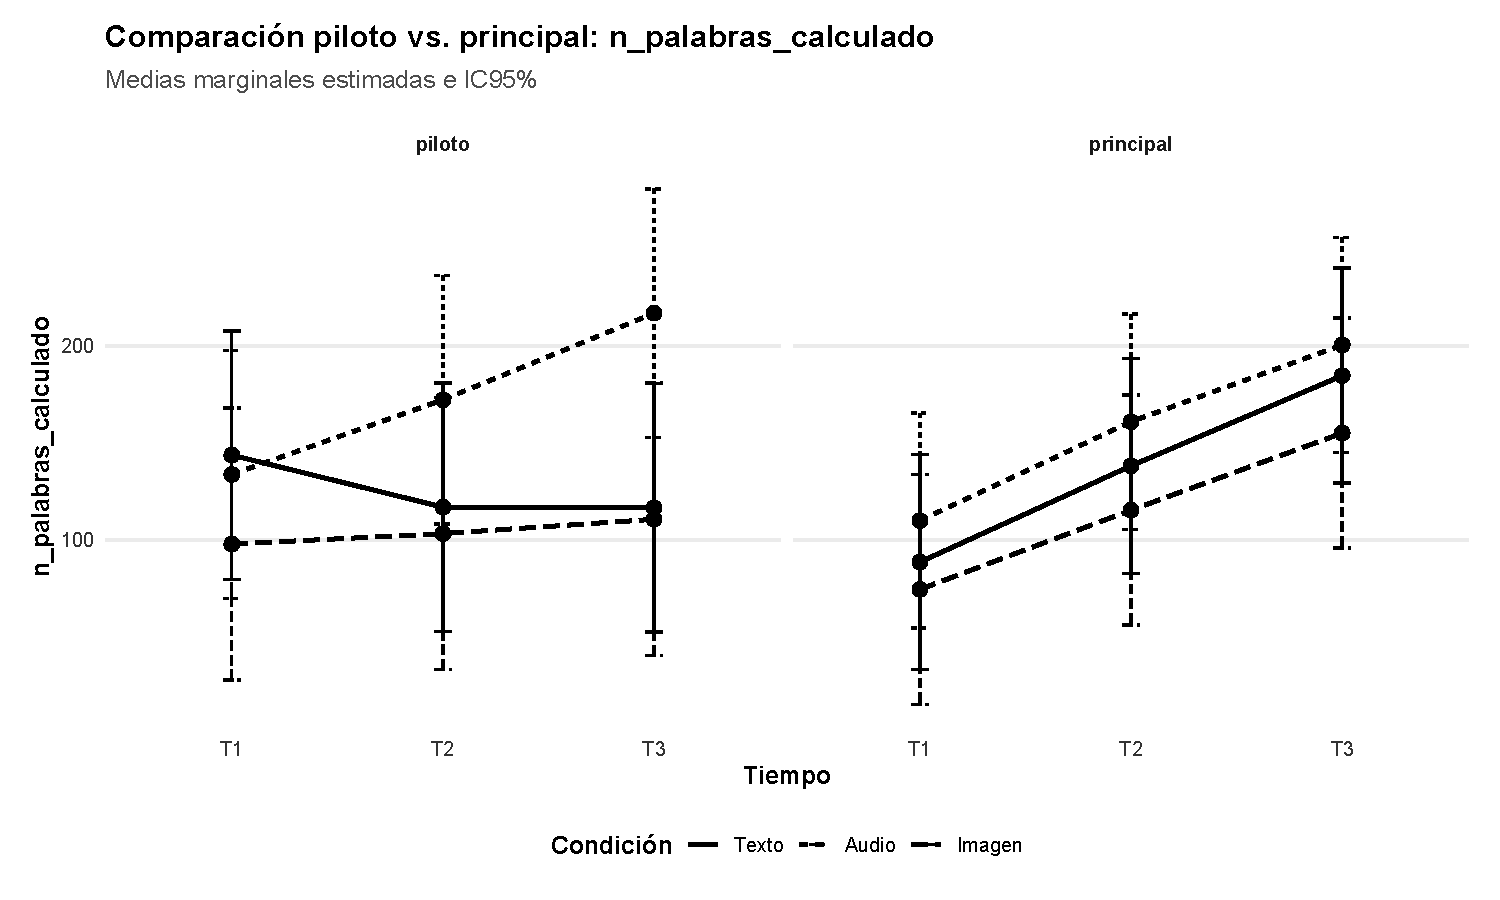
\includegraphics[width=0.95\textwidth]{COMPARACION_n_palabras_calculado_ES.pdf}
	\caption{Medias marginales estimadas de la extensión del texto por cohorte y condición, con
	intervalos de confianza del 95\%. La figura resume el resultado central de la comparación: la
	cohorte principal muestra tres trayectorias ascendentes y paralelas, mientras que en el
	piloto solo la condición Audio asciende y la condición Texto desciende. Las trayectorias no
	son la misma función del tiempo (\texttt{fuente} $\times$ \texttt{tiempo}: $F(2,68) = 6.848$,
	$p = .002$).}
	\label{fig:comparacion}
\end{figure}

\begin{figure}[htbp]
	\centering
	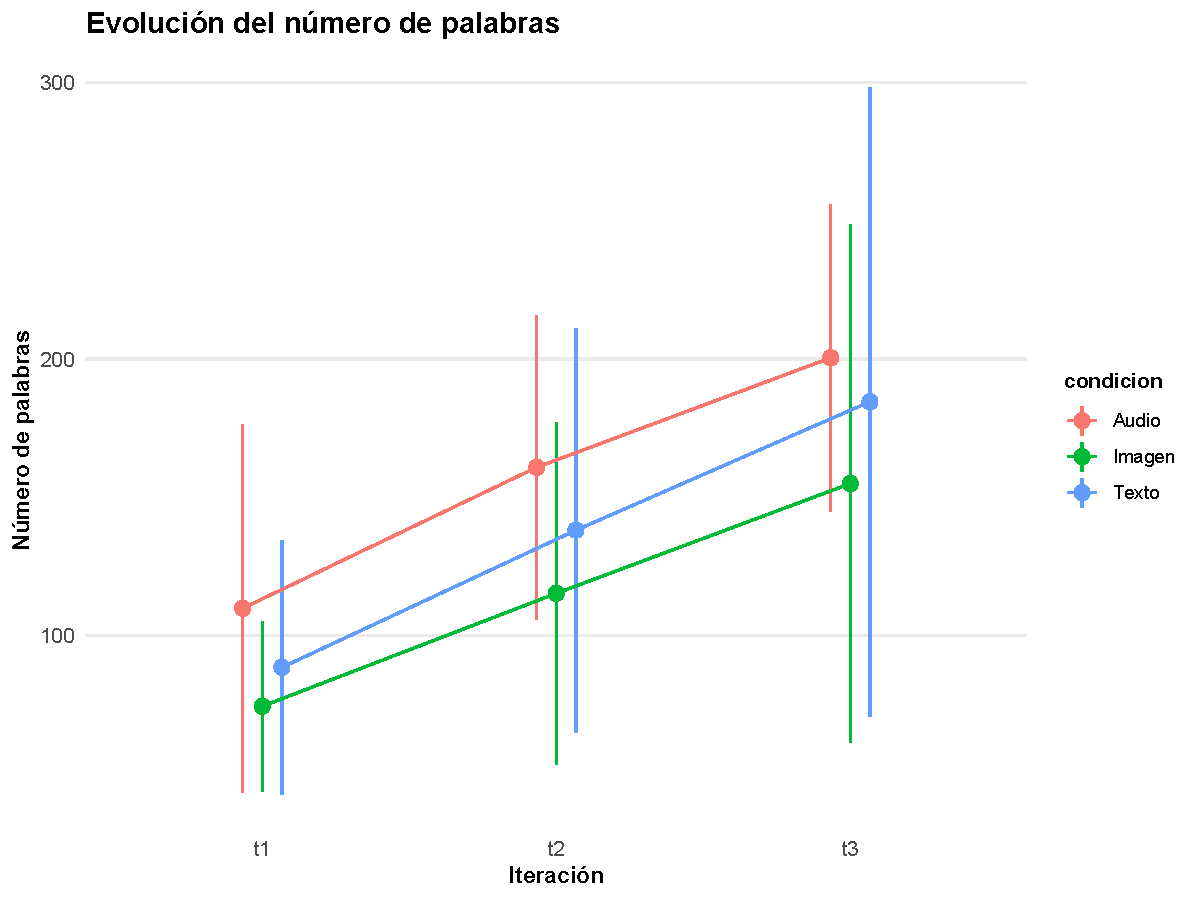
\includegraphics[width=0.95\textwidth]{figura_02_linguistica_es.pdf}
	\caption{Evolución del número de palabras por condición (medias con intervalos de confianza
	del 95\%). Conjunto combinado. La figura reproduce, sin separar cohortes, el efecto de tiempo
	del modelo combinado; debe leerse junto con la Figura~\ref{fig:comparacion}, que muestra que
	ese promedio esconde dos patrones distintos.}
	\label{fig:combinado_linguistica}
\end{figure}

\begin{figure}[htbp]
	\centering
	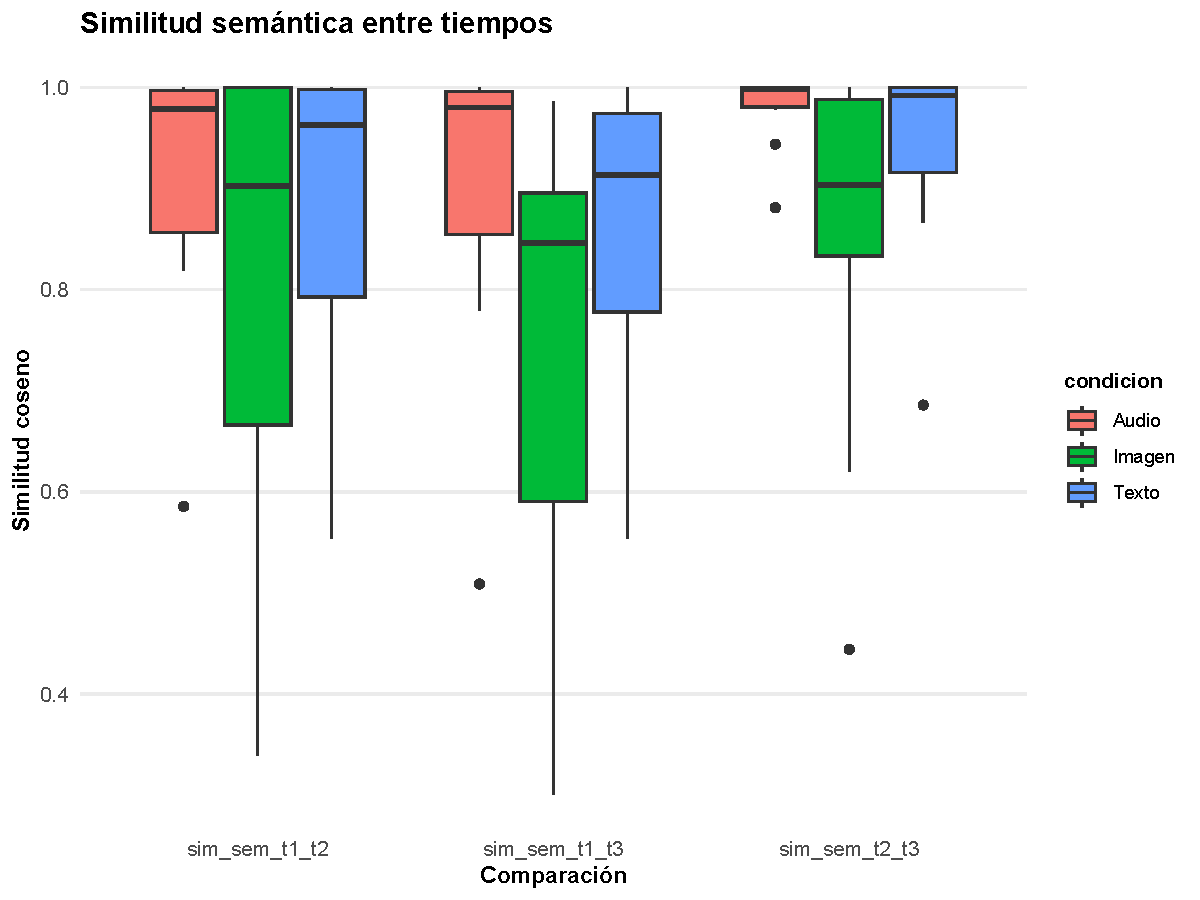
\includegraphics[width=0.95\textwidth]{figura_04_similitud_es.pdf}
	\caption{Similitud semántica (coseno) entre textos sucesivos, por condición. Conjunto
	combinado. La similitud es sistemáticamente mayor en la comparación T2--T3, el resultado que
	se repite en las dos cohortes por separado.}
	\label{fig:combinado_similitud}
\end{figure}

\begin{figure}[htbp]
	\centering
	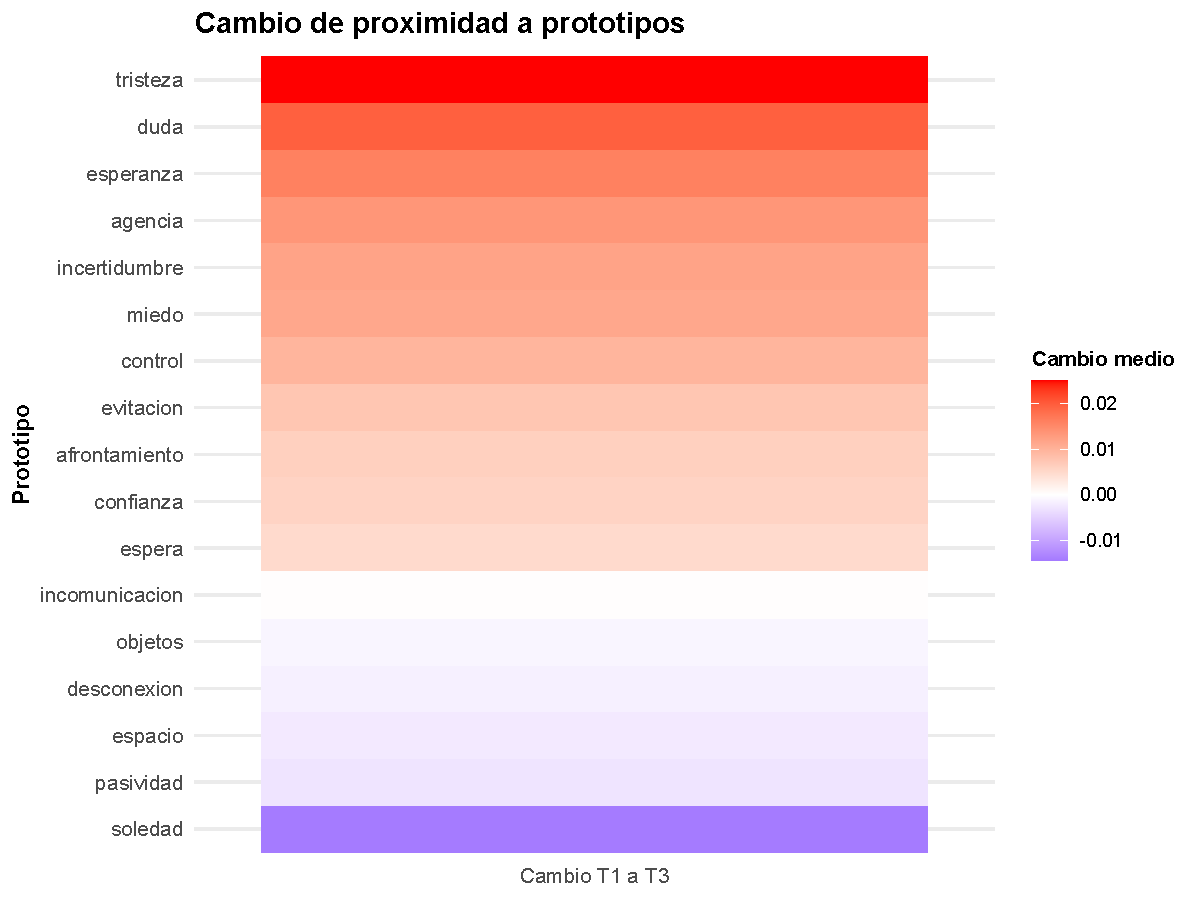
\includegraphics[width=0.95\textwidth]{figura_05_prototipos_es.pdf}
	\caption{Cambio de proximidad a prototipos semánticos entre T1 y T3, por constructo.
	Conjunto combinado ($N = 40$). Los desplazamientos son pequeños y con dispersión mayor que la
	media; la figura no distingue cohortes, y al desagregarlas los patrones difieren.}
	\label{fig:combinado_prototipos}
\end{figure}

\begin{figure}[htbp]
	\centering
	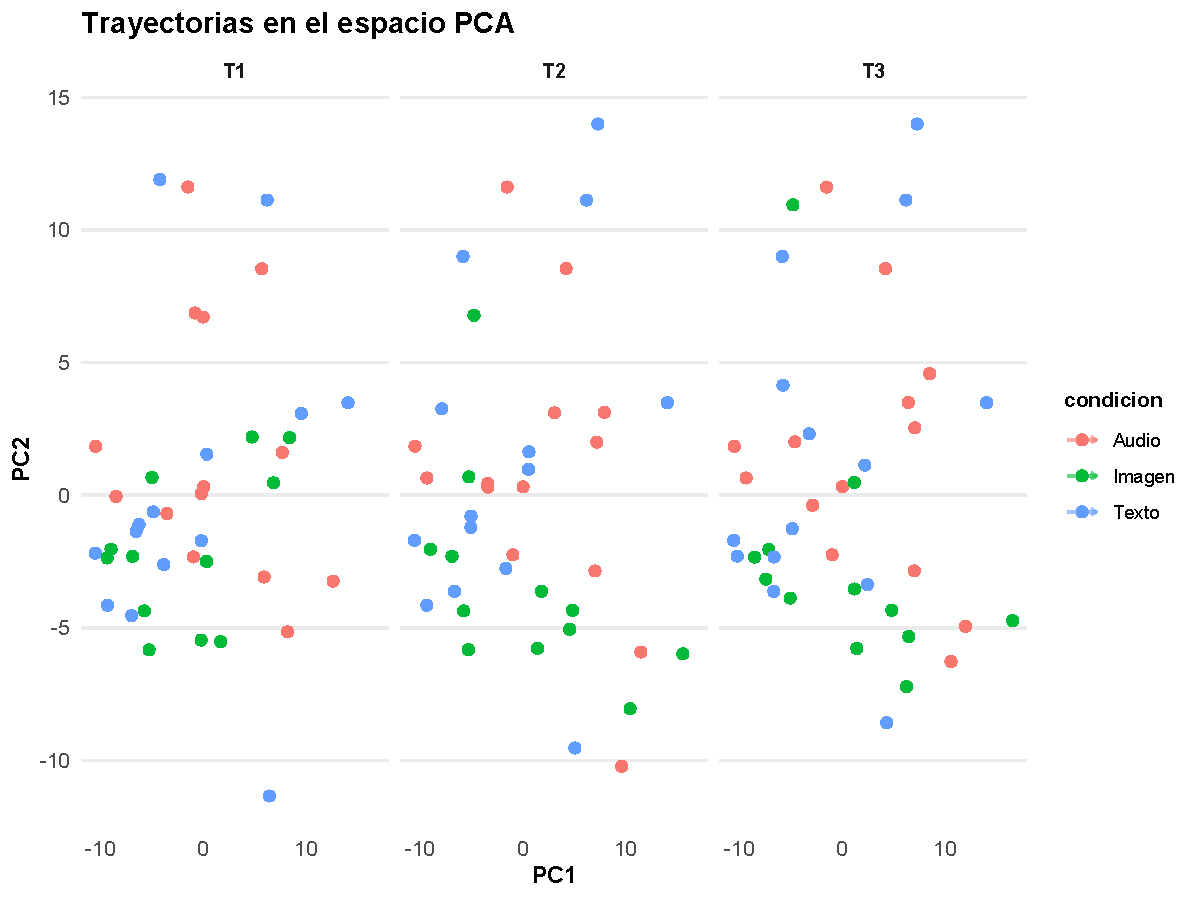
\includegraphics[width=0.95\textwidth]{figura_06_pca_es.pdf}
	\caption{Trayectorias en el espacio de las dos primeras componentes principales (PC1 $=$
	12.68\%, PC2 $=$ 7.51\% de la varianza). Conjunto combinado, 120 textos. Cada participante
	aporta tres puntos unidos por una línea. La varianza explicada es modesta: las distancias en
	este espacio no equivalen a un cambio semántico global.}
	\label{fig:combinado_pca}
\end{figure}

\begin{figure}[htbp]
	\centering
	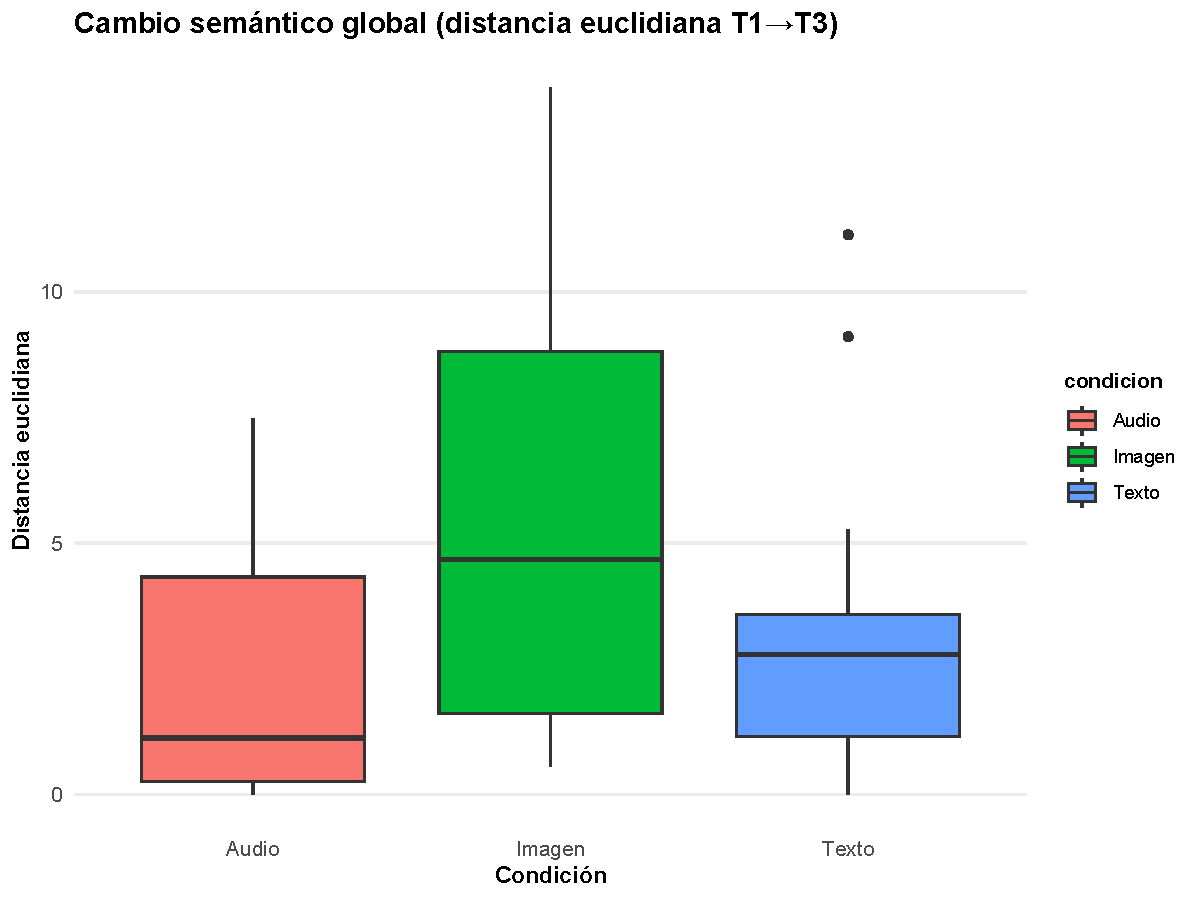
\includegraphics[width=0.95\textwidth]{figura_07_cambio_semantico_es.pdf}
	\caption{Distancia euclidiana T1$\to$T3 en el espacio reducido, por condición. Conjunto
	combinado. La condición Imagen muestra la mayor distancia descriptiva; sin embargo, la
	cohorte principal, analizada por separado, presenta el orden inverso (Texto $<$ Audio $<$
	Imagen con valores mucho menores), lo que ilustra la fragilidad de esta medida.}
	\label{fig:combinado_distancia}
\end{figure}

\begin{figure}[htbp]
	\centering
	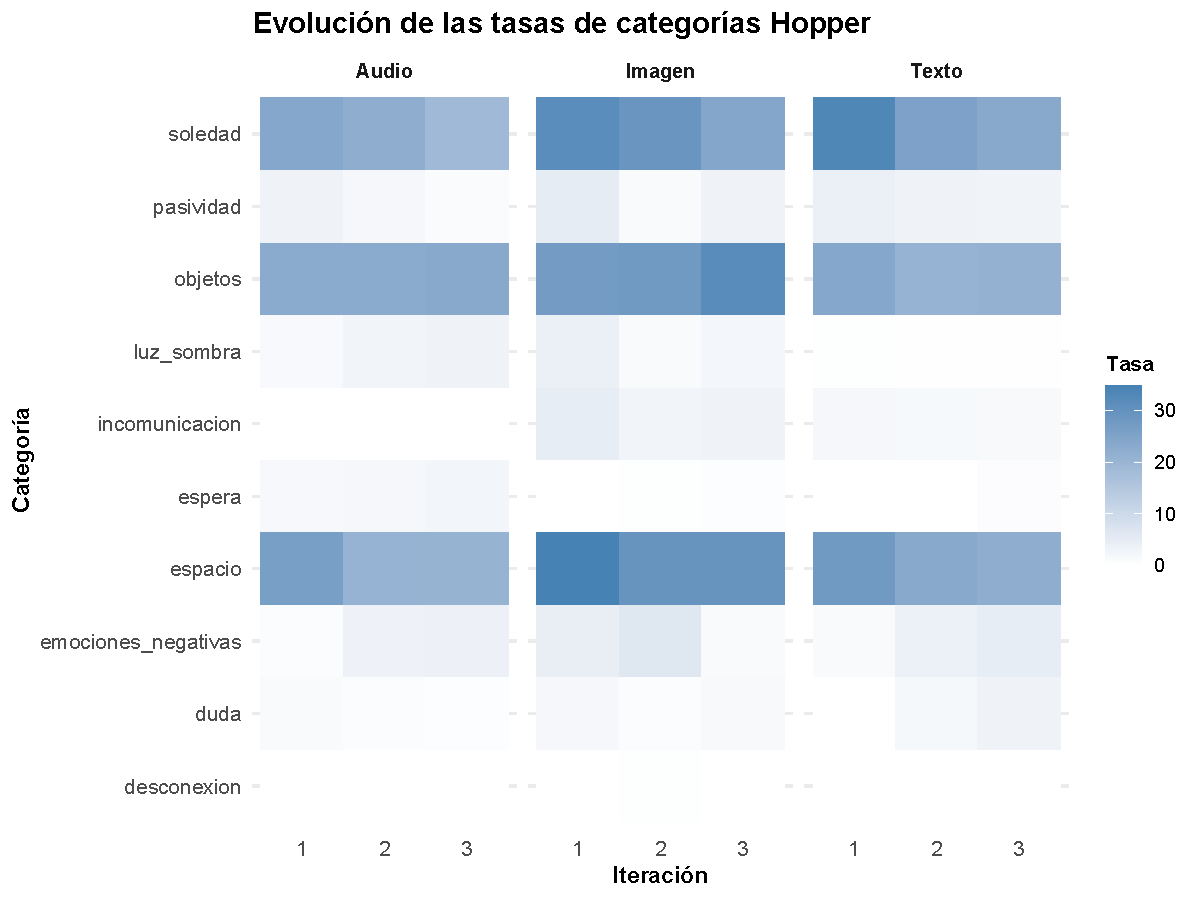
\includegraphics[width=0.95\textwidth]{figura_03_hopper_es.pdf}
	\caption{Tasas por 1000 palabras de los diccionarios temáticos, por condición y momento
	(mapa de calor). Conjunto combinado. Los temas nucleares (soledad, espacio, objetos) dominan
	la densidad léxica; los temas instrumentales y, en particular, \emph{desconexión} e
	\emph{incomunicación}, apenas registran actividad.}
	\label{fig:combinado_hopper}
\end{figure}

\begin{figure}[htbp]
	\centering
	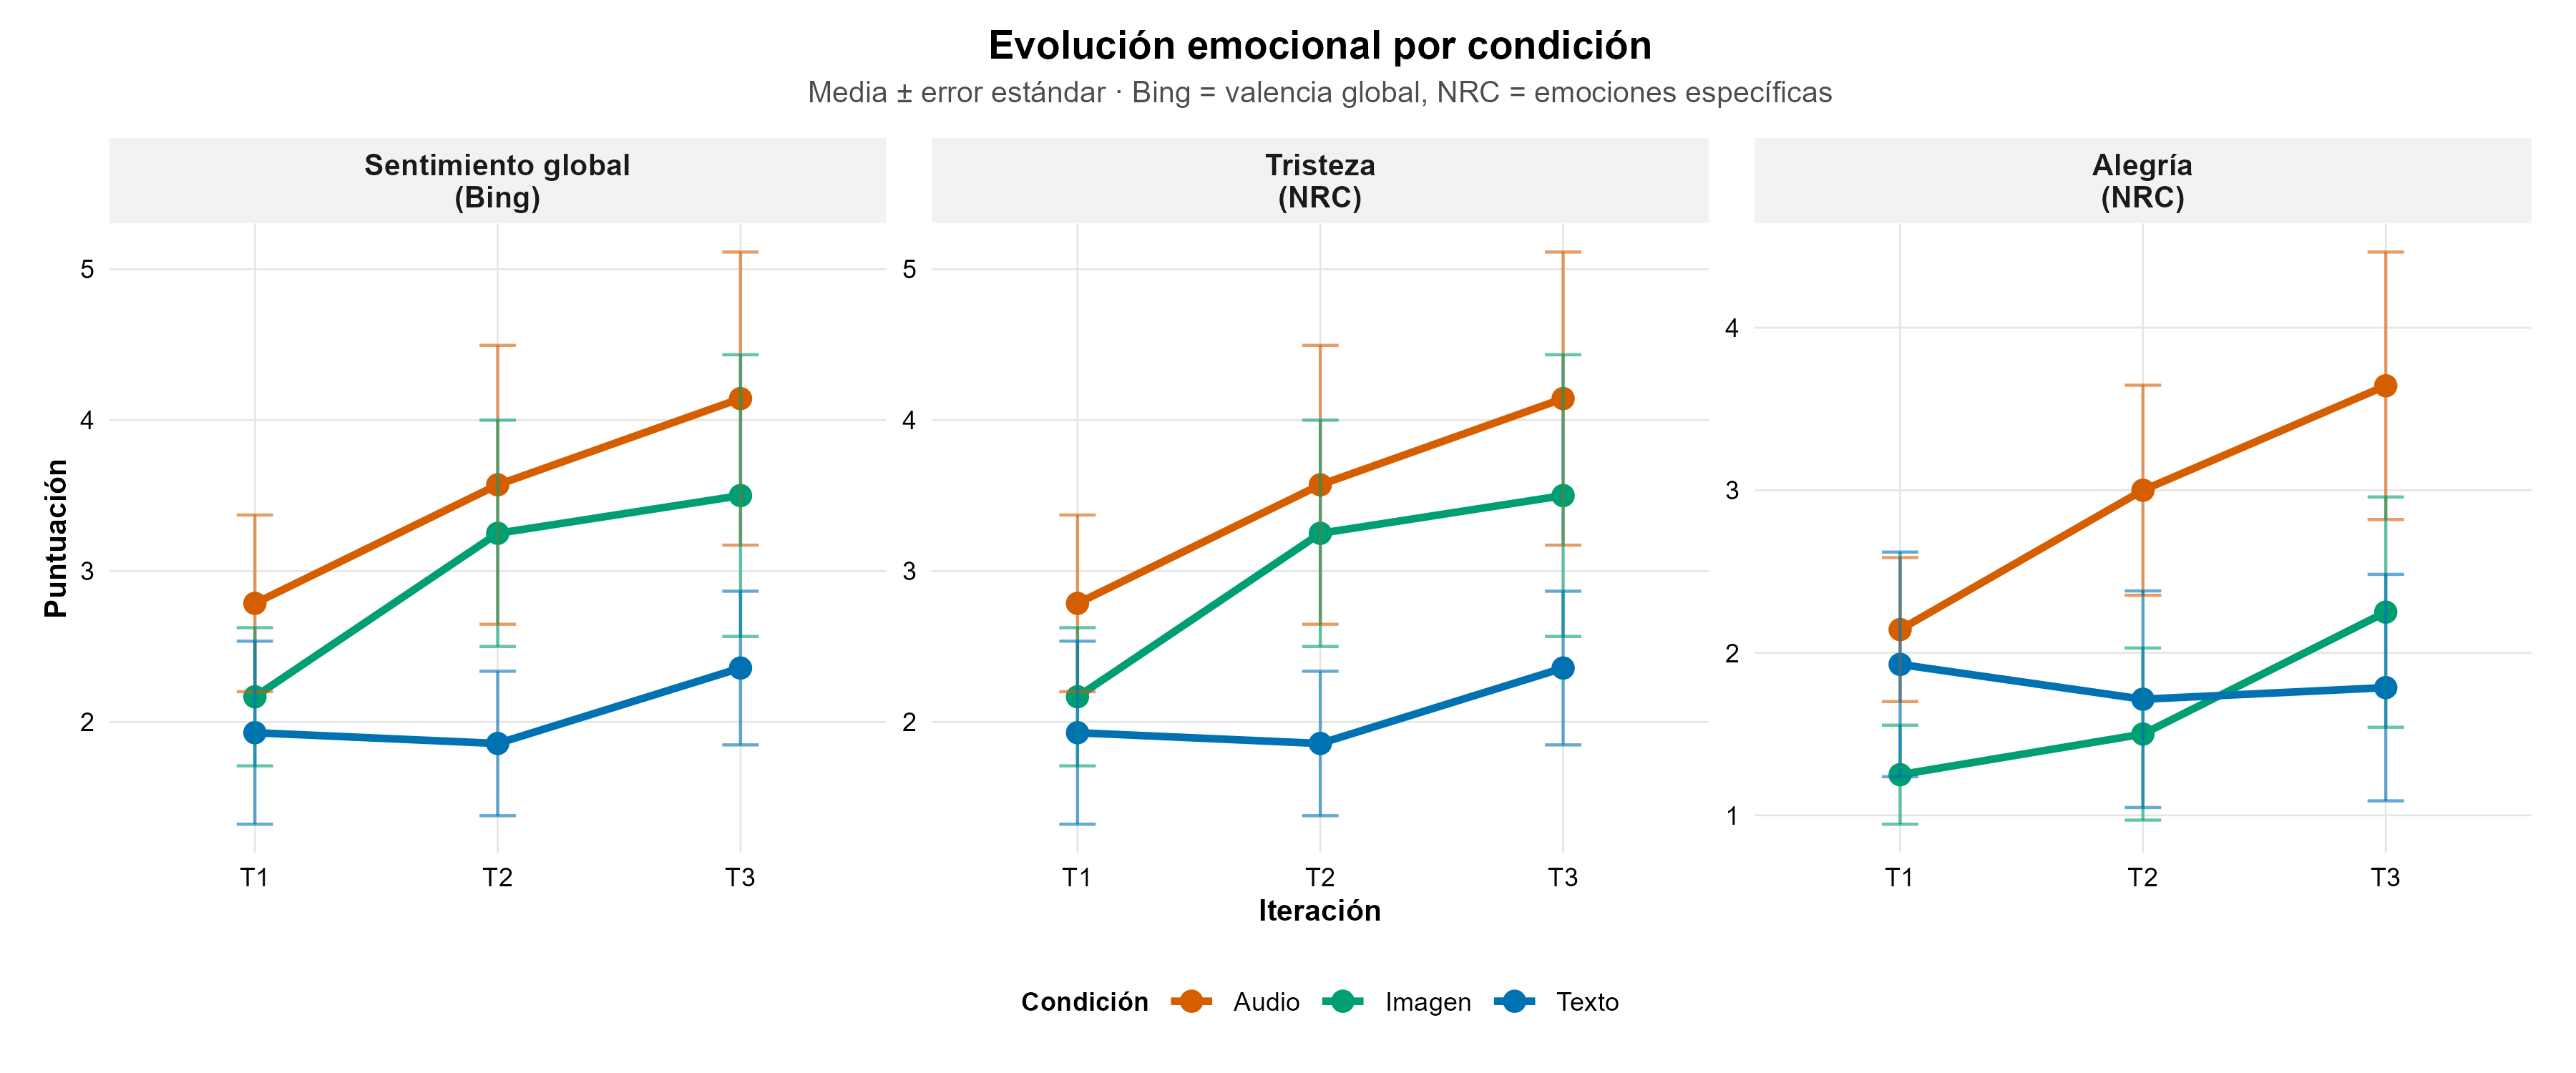
\includegraphics[width=0.95\textwidth]{fig3_emociones.png}
	\caption{Evolución de las emociones medidas con el léxico NRC (tristeza y alegría) y del
	sentimiento global, por condición. Conjunto combinado. \textbf{Advertencia}: el pipeline
	nunca calculó una medida de valencia global tipo Bing/VADER; en las figuras que la solicitan
	se usa \emph{tristeza} como duplicado declarado, de modo que el panel rotulado como
	sentimiento global no aporta información independiente.}
	\label{fig:combinado_emociones}
\end{figure}

\begin{figure}[htbp]
	\centering
	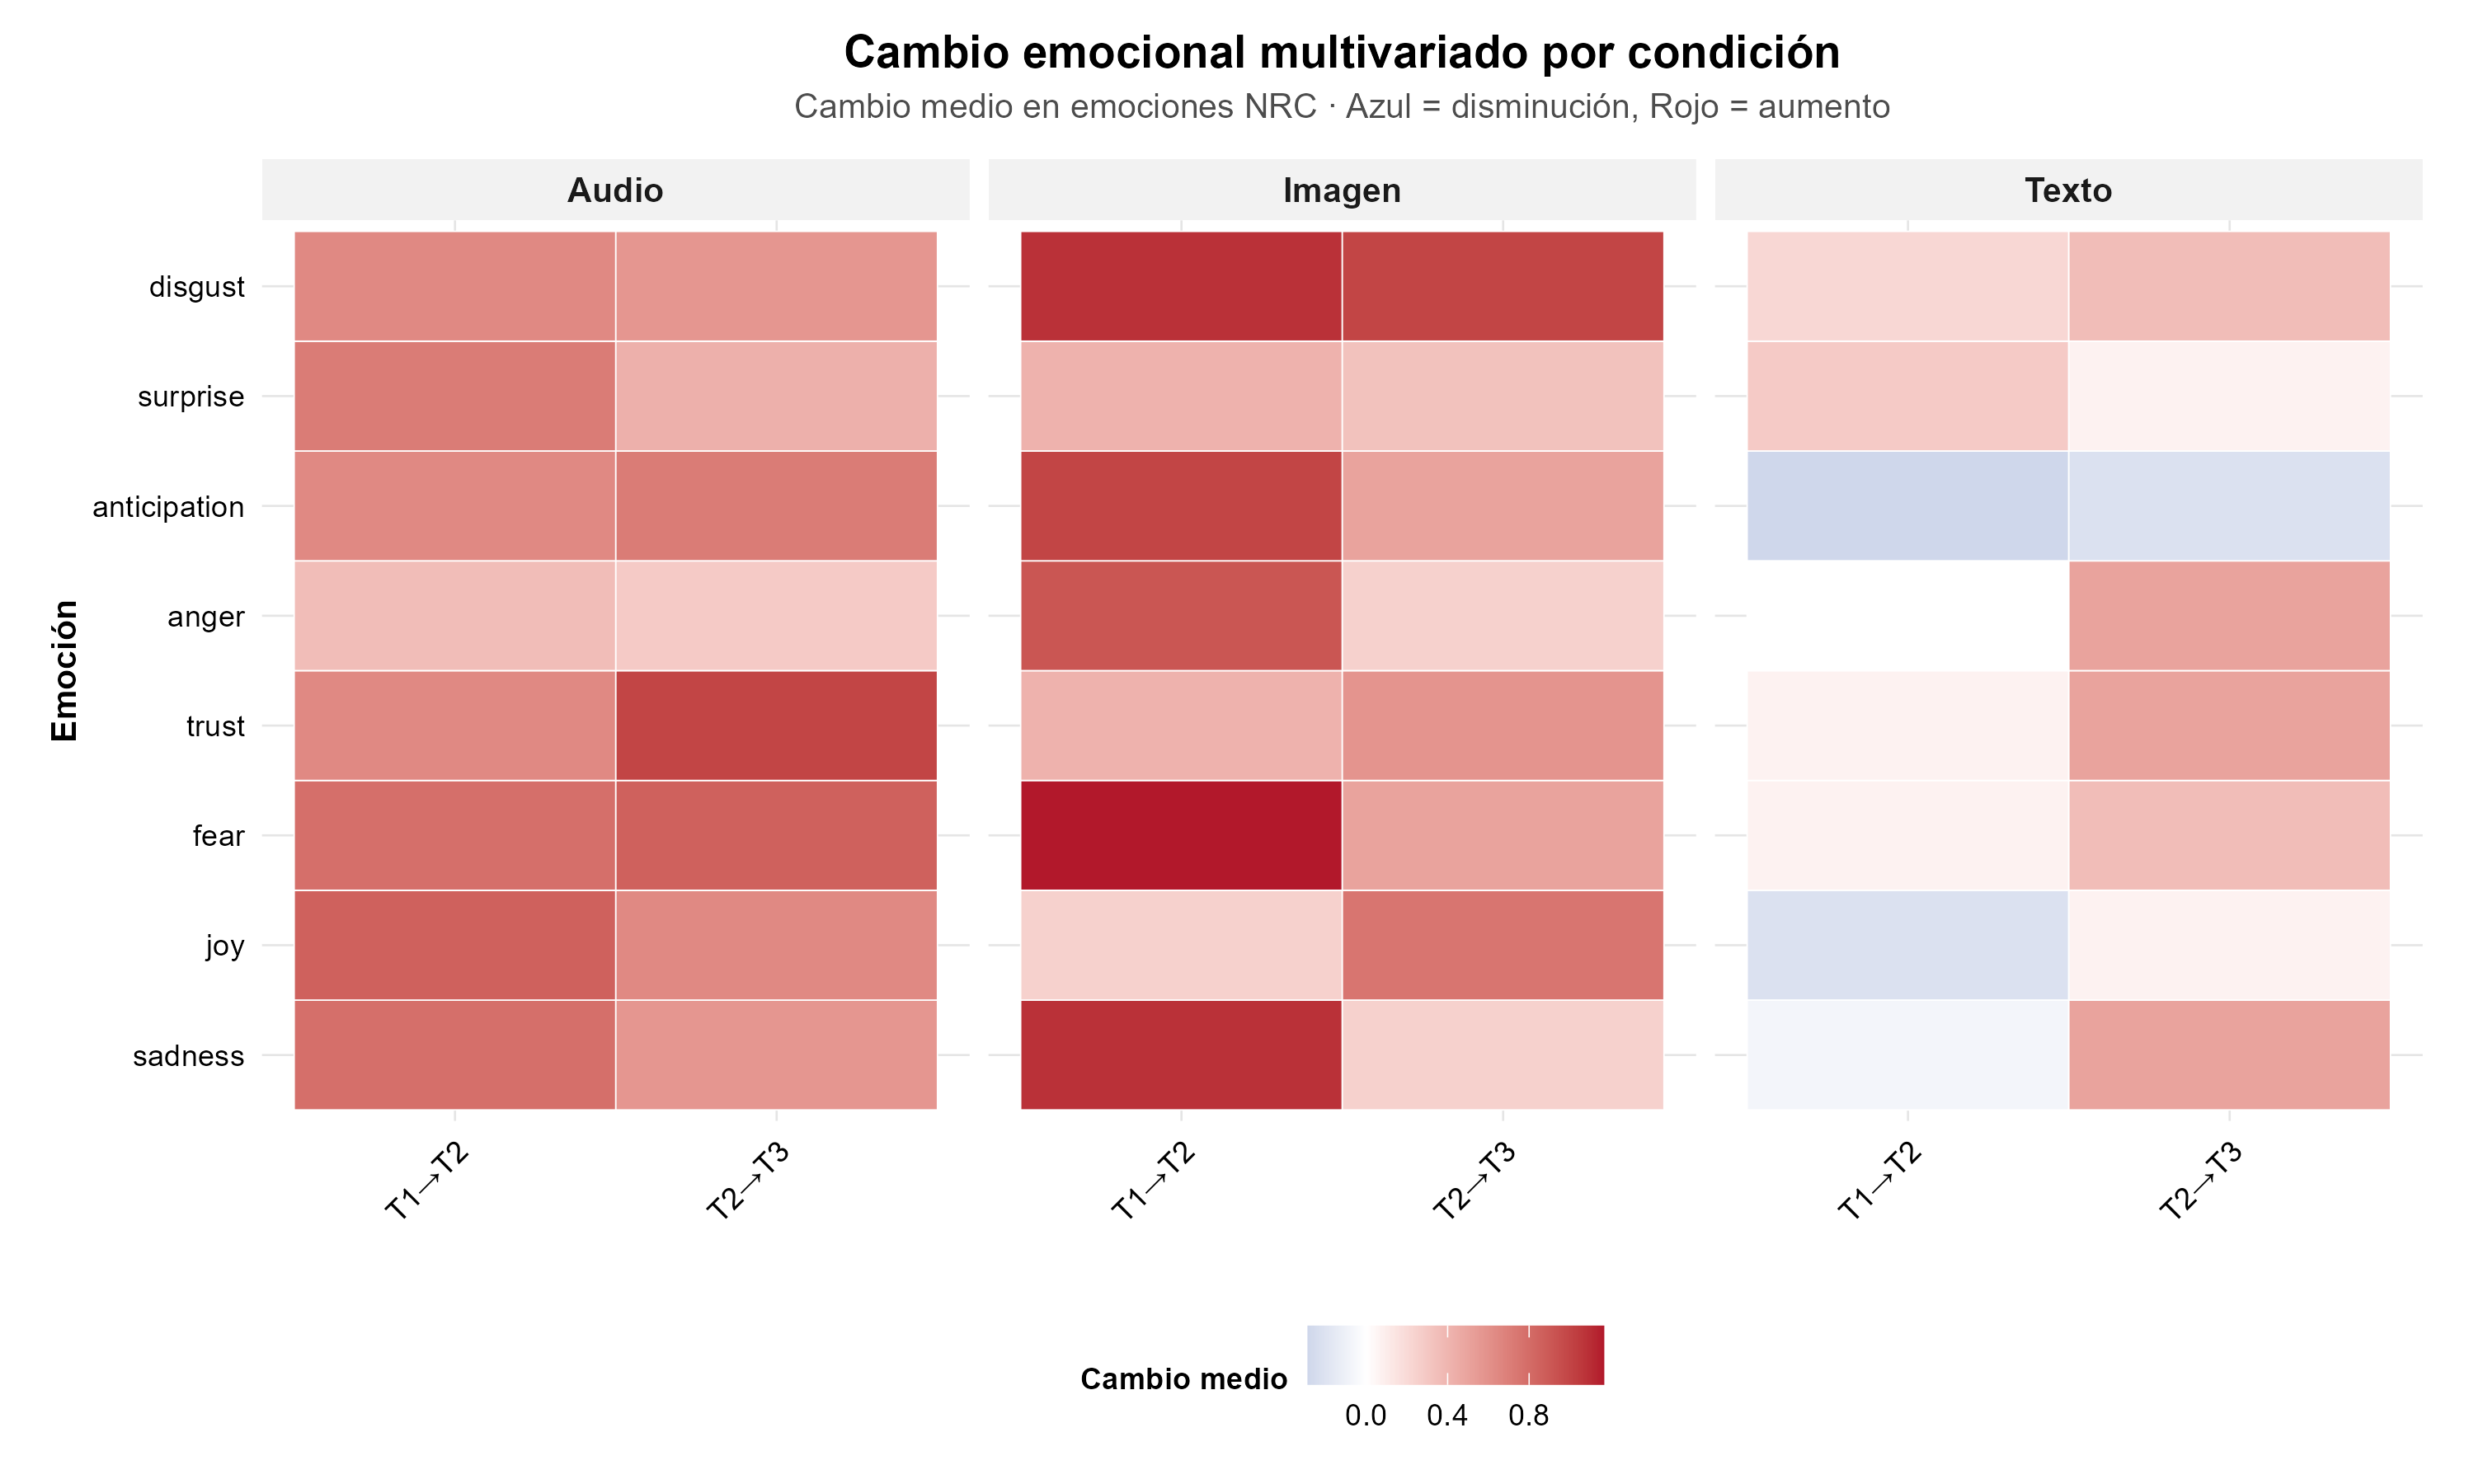
\includegraphics[width=0.95\textwidth]{fig12_cambio_emocional_multivariado.png}
	\caption{Cambio emocional multivariado por condición (mapa de calor de las ocho emociones del
	léxico NRC, en los pasos T1$\to$T2 y T2$\to$T3). Conjunto combinado. Azul indica descenso y
	rojo aumento. Los cambios son de magnitud reducida y no se sometieron a corrección por
	comparaciones múltiples.}
	\label{fig:combinado_cambio_emocional}
\end{figure}

\begin{figure}[htbp]
	\centering
	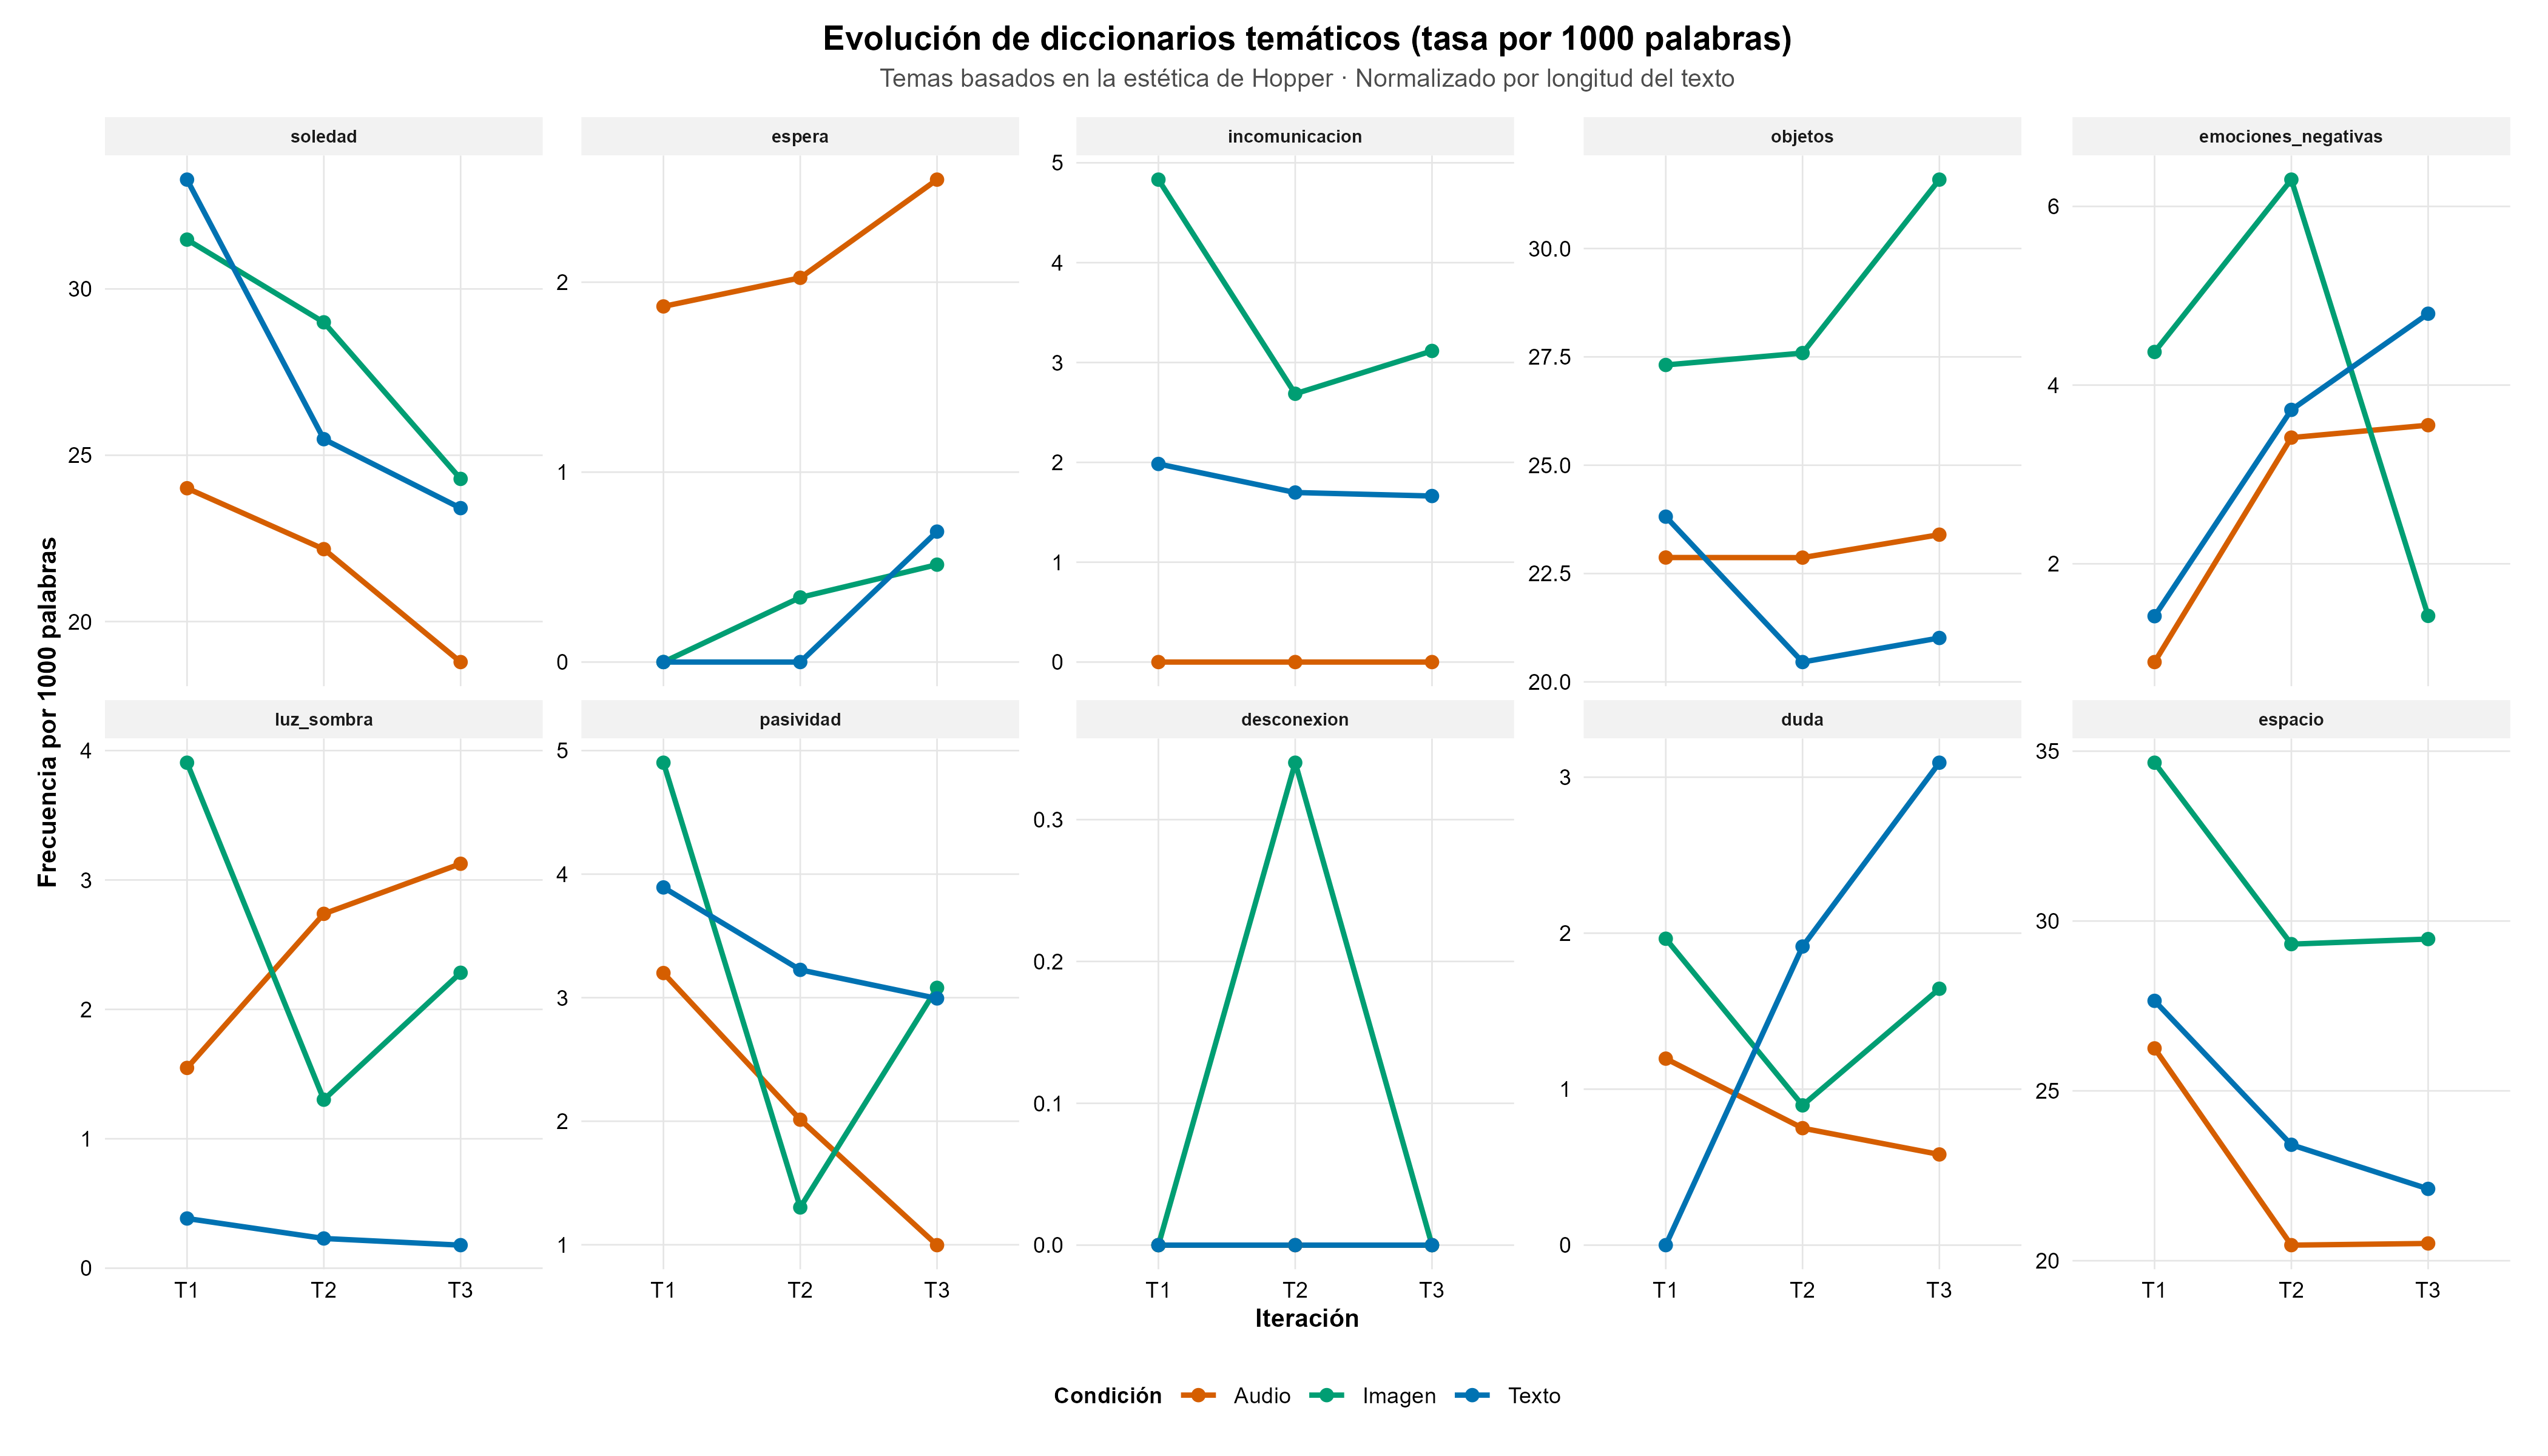
\includegraphics[width=0.95\textwidth]{fig13_diccionarios_tematicos.png}
	\caption{Evolución de las tasas de los diccionarios temáticos por condición, con detalle por
	tema. Conjunto combinado. La figura permite ver que el perfil temático se mantiene estable en
	el conjunto, con oscilaciones dentro del rango de la dispersión individual.}
	\label{fig:combinado_diccionarios}
\end{figure}

\begin{figure}[htbp]
	\centering
	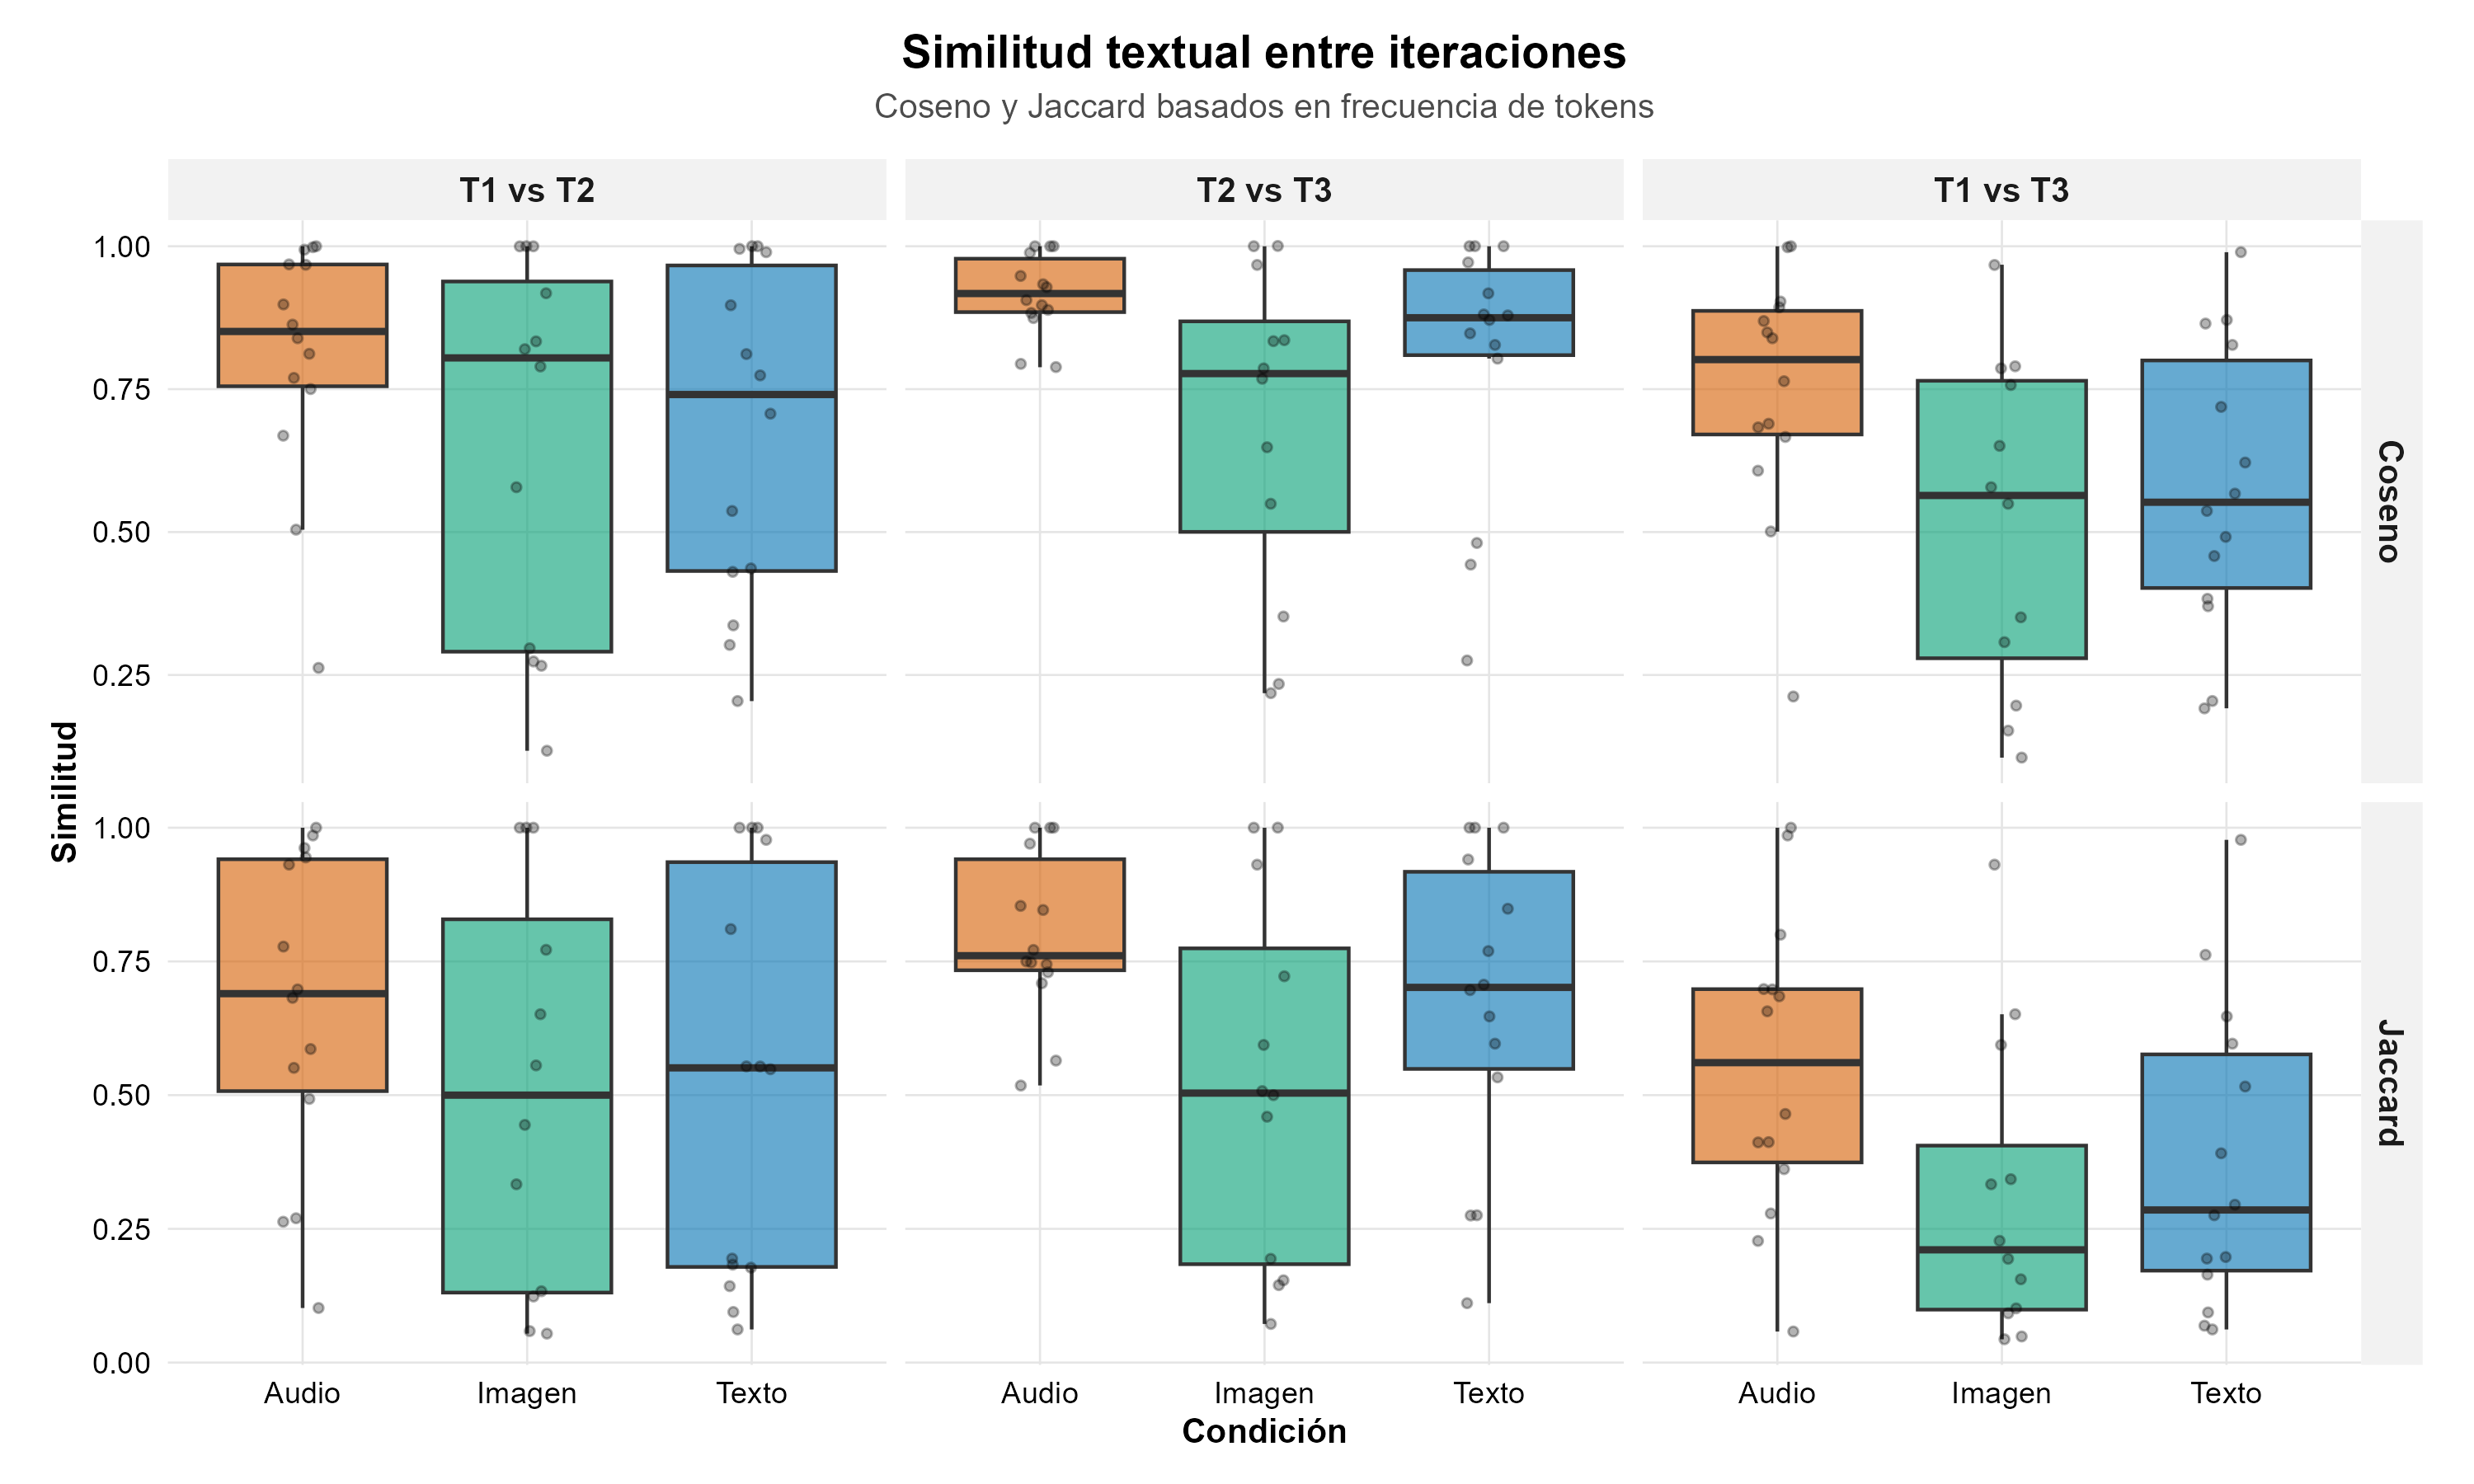
\includegraphics[width=0.95\textwidth]{fig14_similitud_textual.png}
	\caption{Similitud textual entre iteraciones medida con dos indicadores (coseno y Jaccard
	sobre tokens), por condición y par de comparación. Conjunto combinado. La coincidencia de
	ambos indicadores en el ordenamiento de los pares refuerza la lectura de estabilización entre
	T2 y T3.}
	\label{fig:combinado_similitud_textual}
\end{figure}

\begin{figure}[htbp]
	\centering
	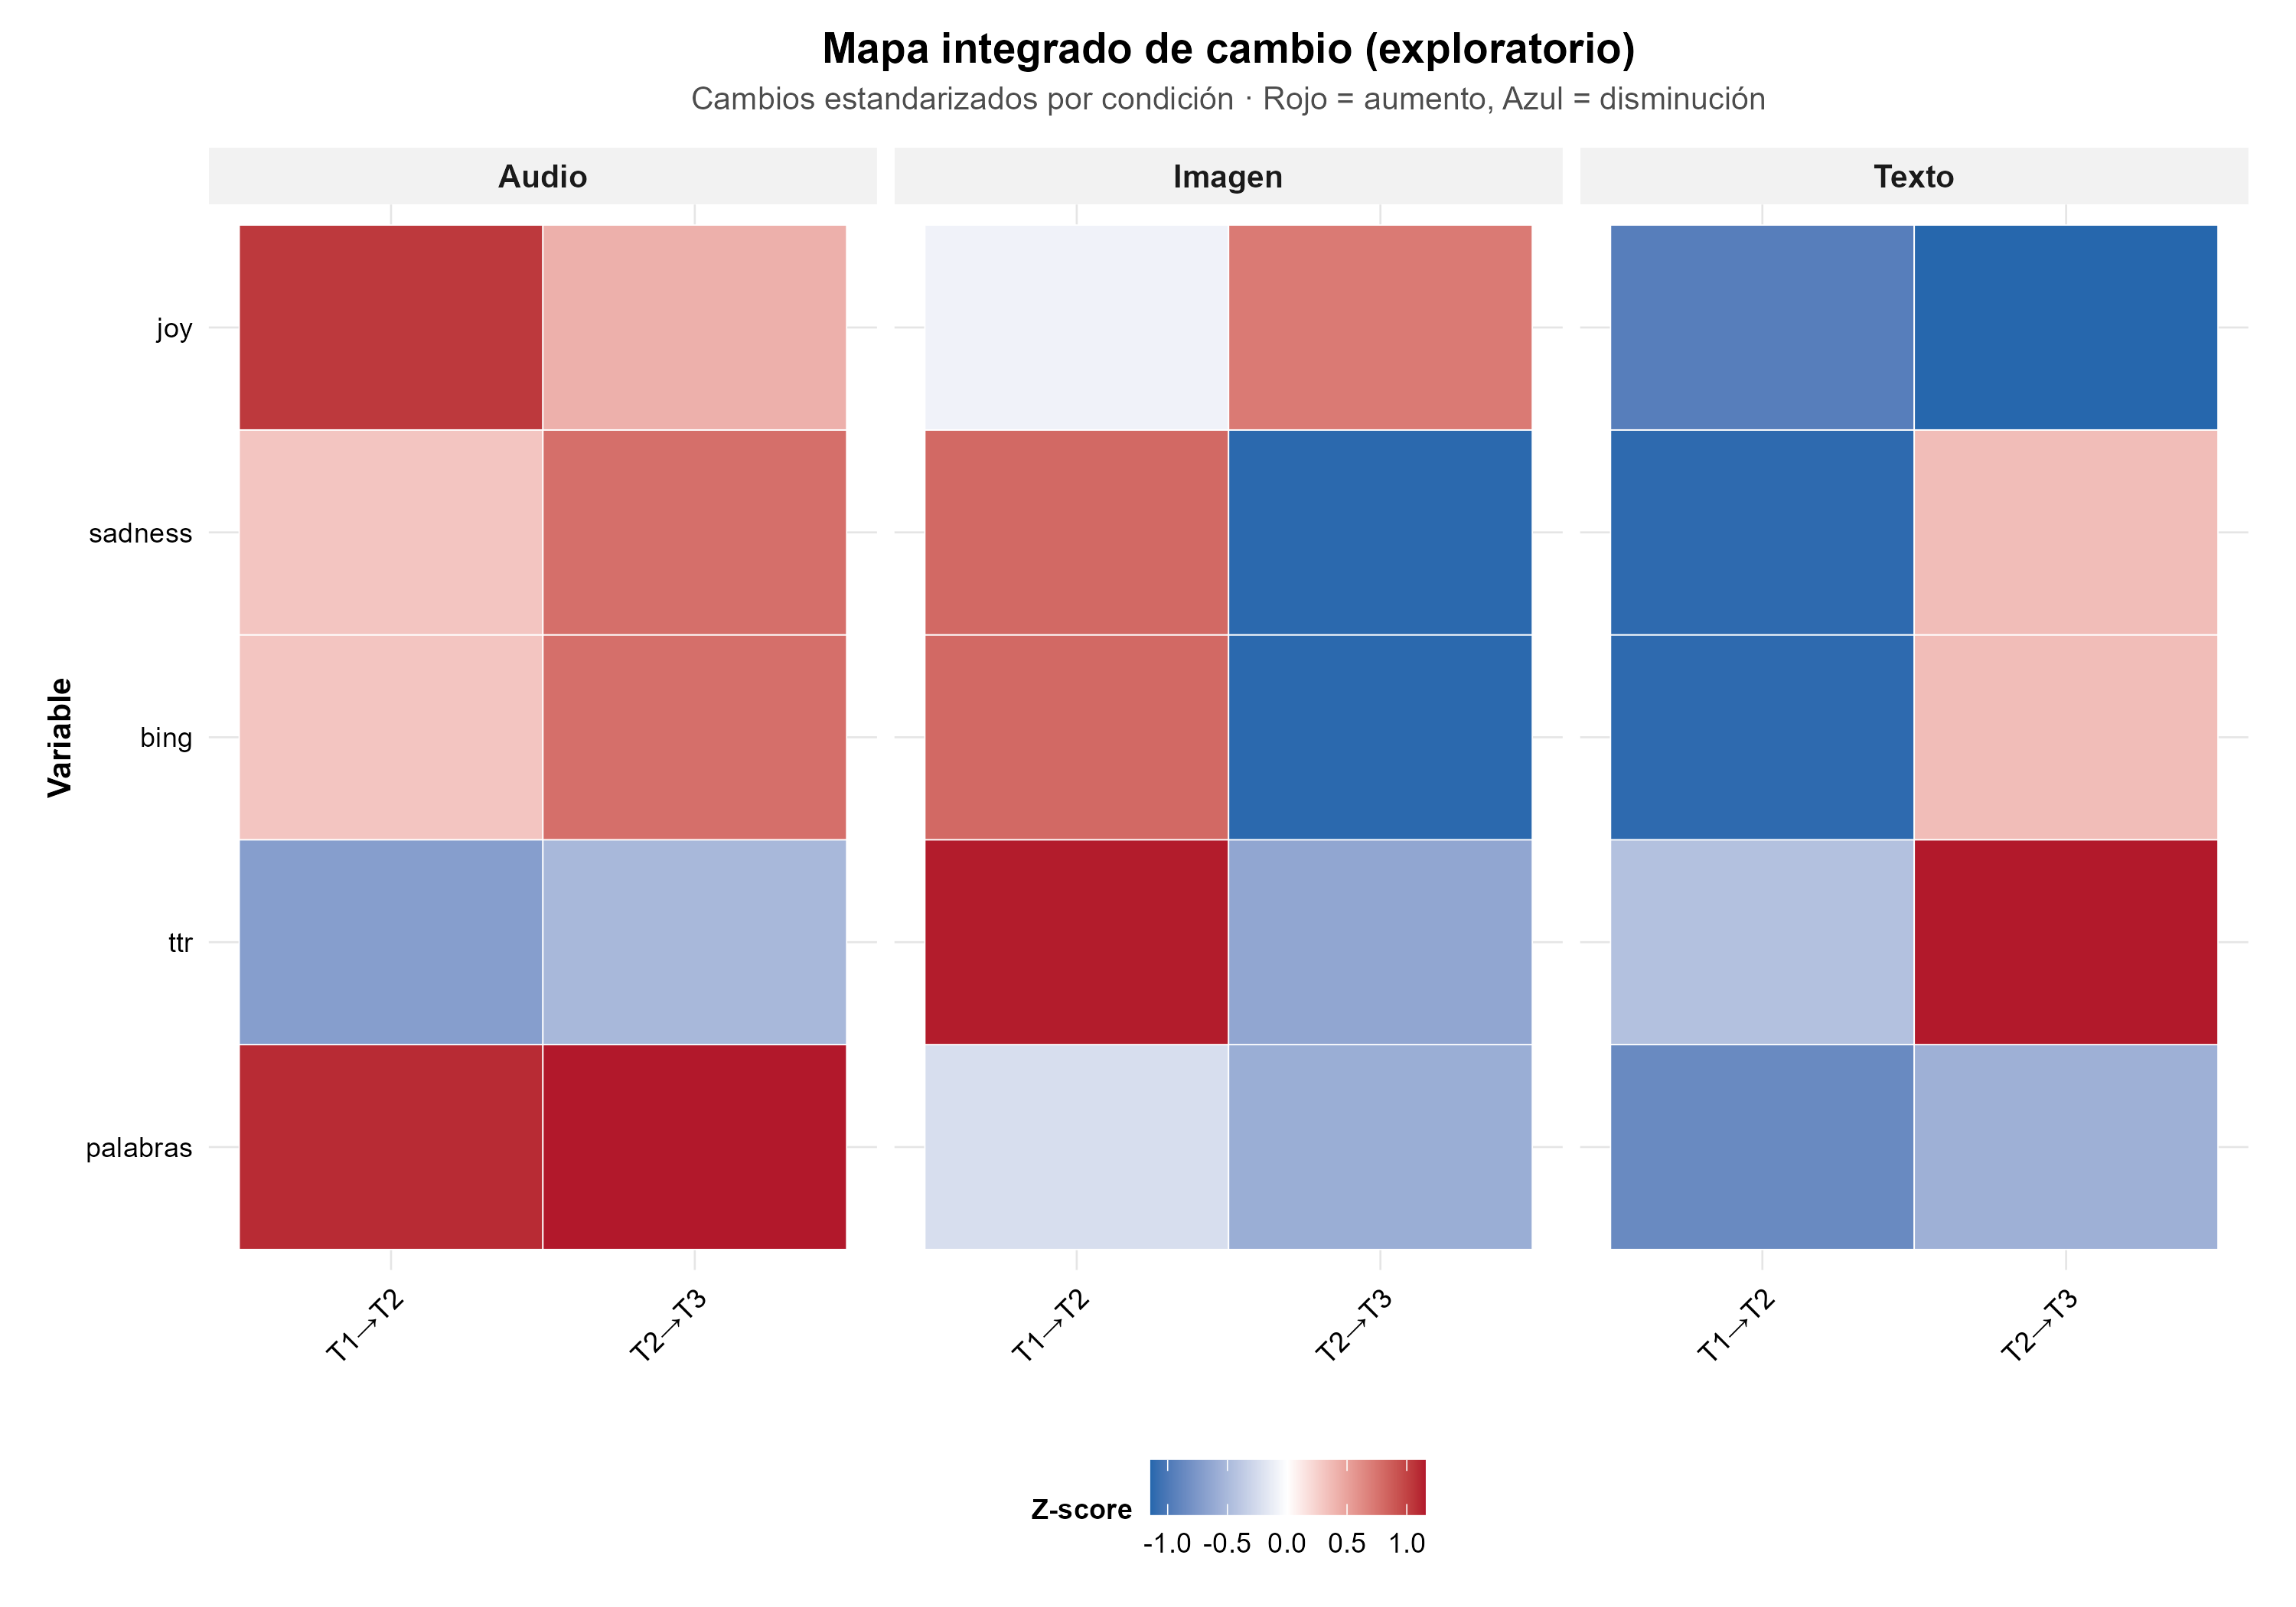
\includegraphics[width=0.95\textwidth]{fig15_mapa_integrado_cambio.png}
	\caption{Mapa integrado de cambio: valores estandarizados (puntuaciones $z$) de los cambios
	en extensión, diversidad léxica y emociones, por condición. Conjunto combinado. Es una figura
	síntesis de carácter exploratorio; los valores se estandarizaron dentro de cada variable y no
	deben leerse como tamaños de efecto.}
	\label{fig:combinado_mapa}
\end{figure}

\begin{figure}[htbp]
	\centering
	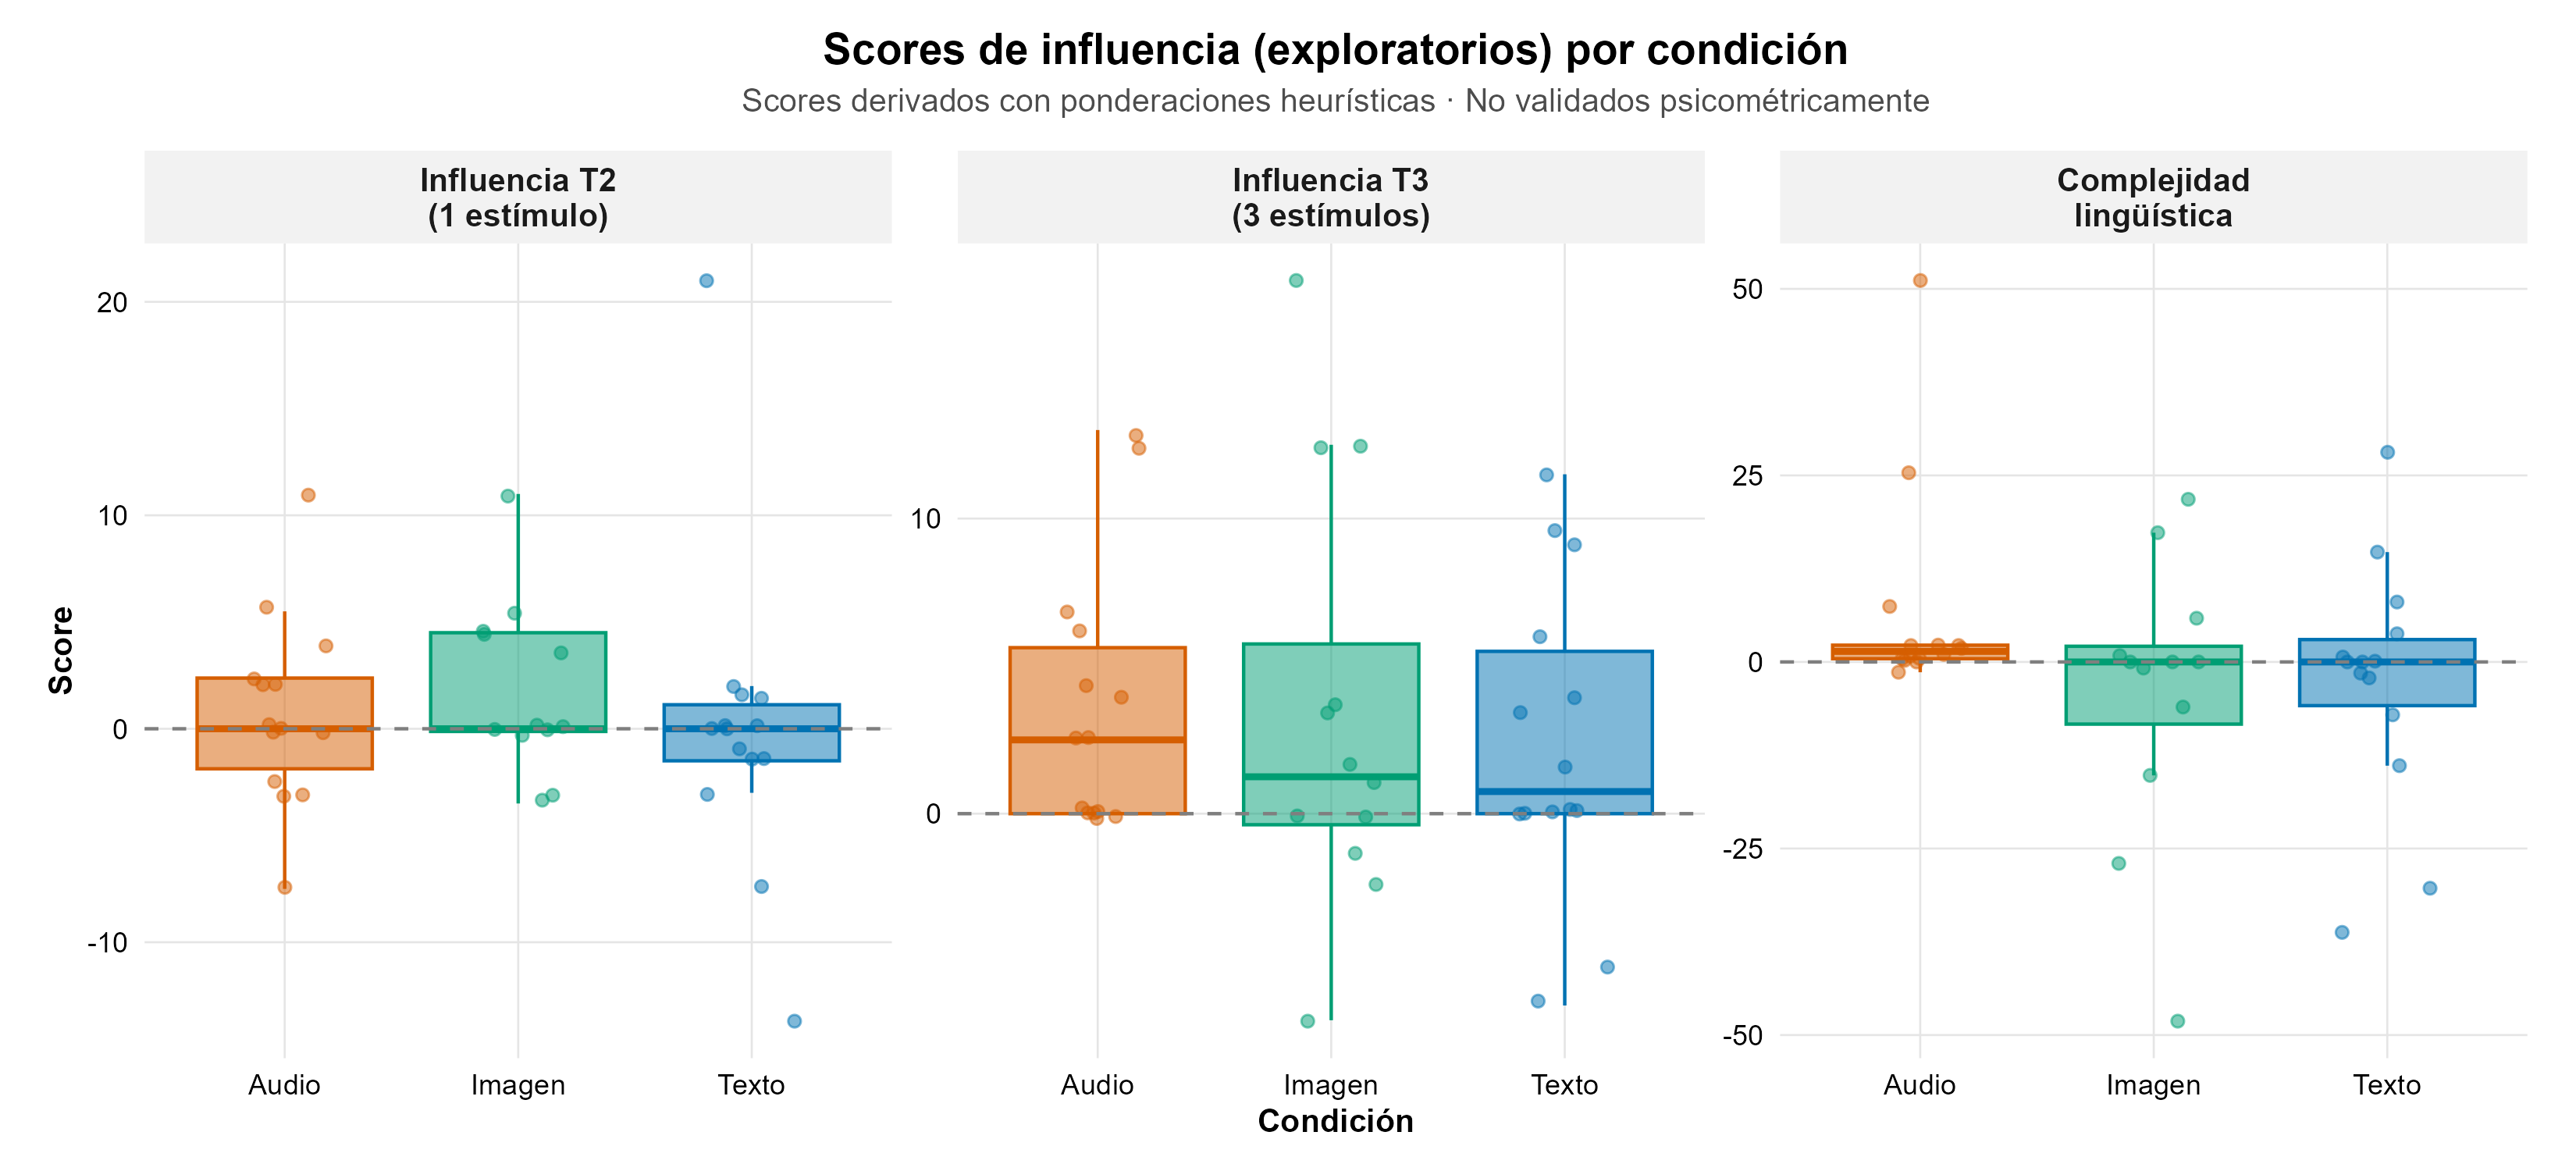
\includegraphics[width=0.95\textwidth]{fig6_scores.png}
	\caption{Puntuaciones heurísticas de influencia y complejidad por condición (T2 y T3).
	Conjunto combinado. Estas puntuaciones se construyen con pesos fijados en el propio código
	del análisis —no derivados de los datos ni validados psicométricamente—, por lo que se
	presentan como indicadores exploratorios de la estructura del texto.}
	\label{fig:combinado_scores}
\end{figure}

\begin{figure}[htbp]
	\centering
	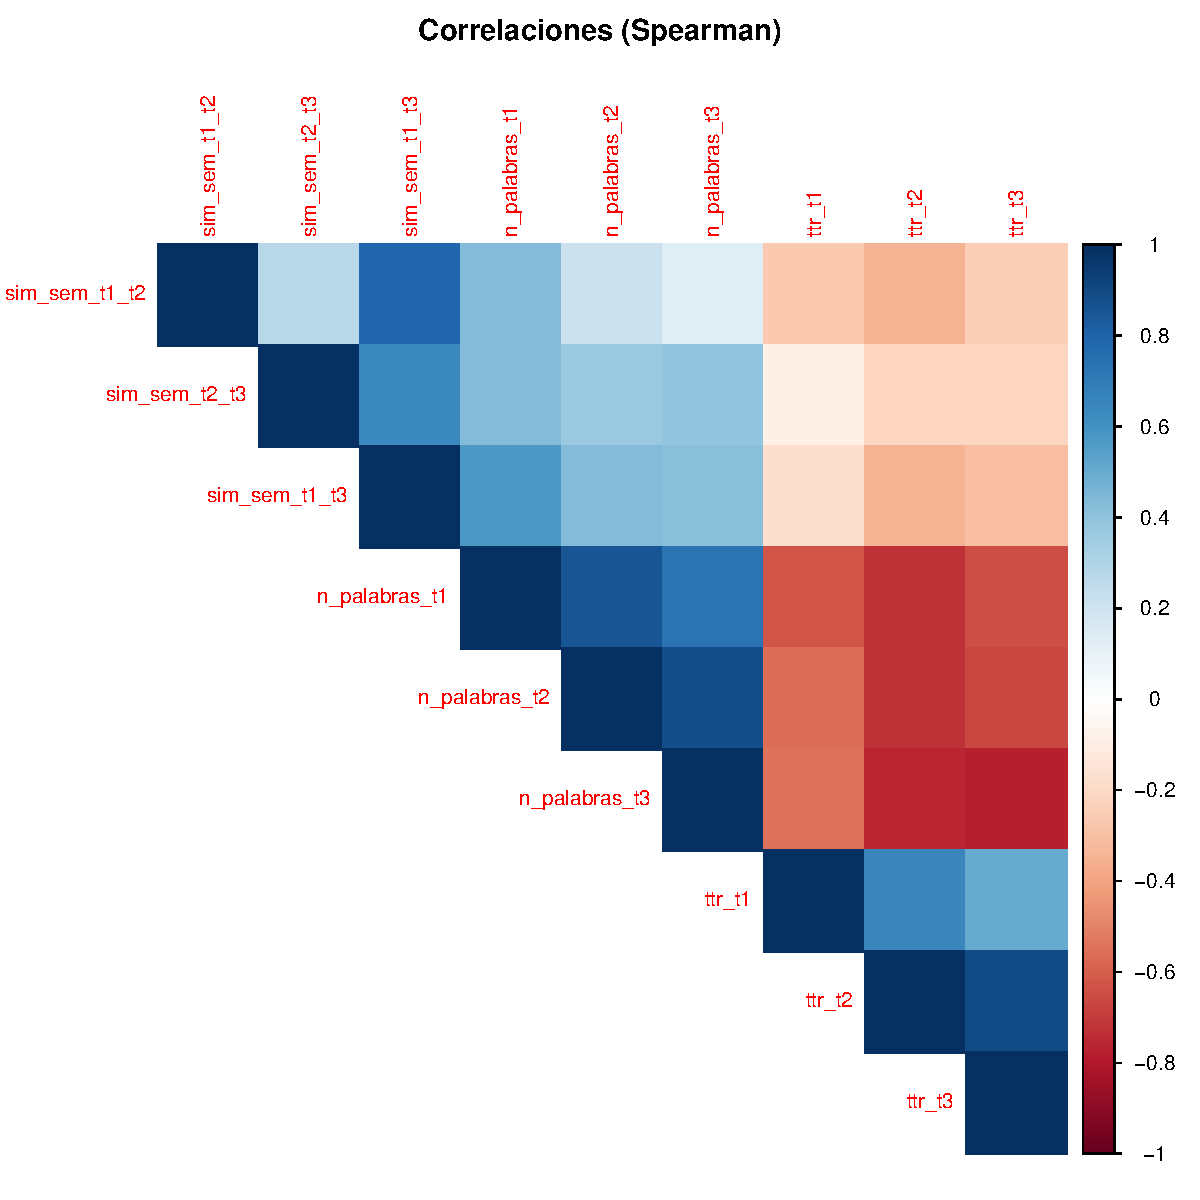
\includegraphics[width=0.95\textwidth]{figura_08_correlaciones_es.pdf}
	\caption{Matriz de correlaciones (Spearman) entre las principales variables del conjunto
	combinado: similitud semántica en los tres pares, número de palabras y diversidad léxica en
	los tres momentos. La asociación negativa entre extensión y diversidad léxica dentro de cada
	momento es la manifestación directa del problema de construcción del TTR discutido en §1.3.}
	\label{fig:combinado_correlaciones}
\end{figure}

\section{Discusión}

\subsection{Qué autoriza y qué no autoriza reunir las dos muestras}

El proyecto dispone de dos cohortes que comparten diseño, tarea y batería de medidas, pero no
muestra ni instrumento. La decisión metodológica que gobierna este documento es explícita:
reunirlas es legítimo para describir \emph{estabilidad de patrones no dependientes del
instrumento} y no lo es para estimar efectos del diseño.

Bajo ese criterio, el conjunto de 40 produce un resultado de valor: la
\textbf{estabilización semántica entre el segundo y el tercer segmento aparece en las dos
cohortes por separado} ($F(2,32) = 5.409$, $p = .0095$ en el piloto;
$F(2,44) = 5.898$, $p = .005$ en el principal). Es un patrón convergente y es, en consecuencia,
el hallazgo más robusto del proyecto: no depende de la muestra, del instrumento ni de la
potencia relativa de cada cohorte.

En cambio, cuando el conjunto se usa para promediar contenido —prototipos, temas, distancias
semánticas—, el promedio no representa a ninguna de las dos muestras. Los desplazamientos de
prototipos del piloto (tristeza $+0.048$, emociones negativas $+0.045$) y del principal
(agencia $+0.026$, duda $+0.023$) difieren en dirección y en constructo; la tabla combinada, que
los promedia, describe un individuo promedio que no existe. La regla práctica que se desprende
es que \textbf{el conjunto combinado sirve para contrastar la forma de un patrón, no para
resumir su contenido}.

\subsection{El tiempo y su régimen: dos formas de trayectoria}

El resultado central de la comparación —nivel sin diferencias ($p = .939$), trayectorias
distintas ($p = .002$)— admite una formulación que el marco teórico del artículo permite leer
con provecho: la \emph{forma} del efecto de la exposición repetida no es una propiedad fija del
procedimiento, sino que depende de la muestra. En la cohorte principal el patrón es aditivo y
general: todas las condiciones crecen (81 a 96 palabras de T1 a T3). En el piloto el patrón es
condicional: solo la condición Audio crece y la condición Texto retrocede.

La literatura que el propio artículo revisa ofrece la clave interpretativa para el segundo
patrón. El artículo señala que en la habilitación lingüística de la escritura se ha encontrado
relación con los modos \emph{escuchar} y \emph{observar}, que no forman par con escribir, y que
la interrelación funcional de la escritura se extiende más allá de su par complementario
(López et al., 2019, 2020, citados en López Corral et al., 2024). Un efecto específico de la
condición auditiva es, por tanto, exactamente del tipo que esa línea de investigación haría
esperar, y no un resultado anómalo. El problema es que en el piloto ese efecto no se puede
separar de la fragilidad de una interacción estimada con seis participantes por condición, y que
en la muestra mayor —la que tiene potencia para detectarla— la interacción no aparece
($p = .989$).

La conclusión prudente es que el piloto \textbf{genera} la hipótesis de una habilitación
específica por el modo escuchar y que el principal no la sostiene. Formularla como hallazgo
requeriría un diseño con potencia calculada y con el contraste Audio--Texto declarado de
antemano.

\subsection{Modo reactivo o cantidad de contacto: la pregunta que queda abierta}

El diseño acumula estímulos: un estímulo en T2 y tres en T3. Esta decisión, coherente con la
idea de que la escritura se apoya en lo previamente observado, escuchado o leído, introduce una
confusión que ningún análisis de estos datos puede resolver: el efecto de tiempo es
simultáneamente un efecto del tiempo transcurrido, de la práctica y de la cantidad de contacto
con el referente.

El patrón del principal es compatible con las dos lecturas. Si lo que habilita es el
\emph{modo}, el diseño debería haber mostrado diferencias entre condiciones: no las mostró. Si
lo que habilita es la \emph{cantidad de contacto}, el diseño debería mostrar un crecimiento
monótono con la acumulación: lo mostró, y de igual magnitud en las tres condiciones. Los datos
favorecen la segunda lectura, pero no la demuestran, porque no hay una condición con contacto
constante que sirva de control. La prueba decisiva es un diseño que manipule la cantidad de
contacto manteniendo el modo fijo —o al revés—, y ese diseño no se ha corrido.

\subsection{Segmentación del episodio y Referente AB}

La convergencia entre cohortes en el patrón semántico —T2--T3 como el par más similar en ambas
muestras— es el resultado que mejor se corresponde con la descripción teórica del segundo
segmento del episodio. El artículo propone que, tras la primera versión escrita, el individuo
interactúa con el referente original y/o con su versión escrita, produciendo un texto que es
una modificación del anterior \emph{a propósito del referente original}, y denomina a ese
producto el \emph{Referente AB} (López Corral et al., 2024). Si el anclaje del episodio se
desplaza efectivamente del referente al texto, el desplazamiento semántico entre el segundo y
el tercer texto debe ser menor que entre el primero y el segundo: es exactamente lo que se
observa, y se observa dos veces.

Sostener esta interpretación con la fuerza que merece exige, sin embargo, algo que estos datos
no aportan: análisis de contenido que muestren que el tercer texto elabora elementos del
segundo y no del referente original. La similitud coseno es compatible con la interpretación,
pero también con la mera continuidad estilística o temática. Es, por tanto, un apoyo parcial con
confianza moderada, no una confirmación.

\subsection{Extensión, diversidad y la lección del indicador}

El contraste entre cohortes en la diversidad léxica es, en términos metodológicos, el resultado
más instructivo del conjunto. El TTR desciende en el principal ($p < .001$) y no en el piloto
($p = .144$), y la diferencia coincide con que en el principal la extensión se duplica y en el
piloto no crece de forma general. La conclusión que se impone es que el descenso del TTR
\textbf{no informa sobre el escritor sino sobre el indicador}: en diseños donde la extensión
varía entre momentos, el TTR deja de ser una medida interpretable de riqueza léxica.

Esto tiene una consecuencia para el marco teórico que conviene explicitar. Si la extensión del
episodio de escritura se va a estudiar con indicadores automáticos, esos indicadores deben ser
robustos a la longitud del texto (por ejemplo, TTR estandarizado a un número fijo de tokens,
medidas de diversidad basadas en modelos, o índices de densidad conceptual sobre unidades
normalizadas). De lo contrario, se corre el riesgo de interpretar como cambio en la
\emph{organización} del contenido lo que es un cambio en su \emph{cantidad}.

\subsection{Contenido: por qué el conjunto no puede sostener afirmaciones}

Los análisis de contenido sobre el conjunto —prototipos, temas, emociones— presentan tres
problemas acumulados: mezclan dos regímenes, no llevan corrección por comparaciones múltiples y
no tienen prueba inferencial asociada. Sus magnitudes, además, son pequeñas: los cambios de
proximidad a prototipos no superan $|\Delta| = 0.025$ con desviaciones mayores que la media. Se
reportan como exploratorios y sirven, sobre todo, para dos cosas: (i) generar hipótesis
específicas que puedan preregistrarse, y (ii) documentar un problema de instrumento, ya que los
diccionarios de \emph{desconexión} e \emph{incomunicación} apenas registran actividad en el
corpus.

Sobre la imaginación, que el artículo desarrolla con detalle —quien imagina se apoya en lo que
ha observado, escuchado o leído, y la forma del contacto previo condiciona el uso imaginativo
del conocimiento (Ryle, 2005, citado en López Corral et al., 2024)—, ninguno de los dos
conjuntos de análisis aporta evidencia concluyente. T3, el momento en que los tres modos están
disponibles, no muestra un desplazamiento de contenido de magnitud apreciable en ninguna de las
medidas empleadas.

\subsection{Robustez: lo que aguanta y lo que no}

\begin{table}[htbp]
	\centering
	\caption{Afirmaciones no sostenibles con el conjunto analizado y alternativas defendibles.}
	\label{tab:no_sostener_combinado}
	\small
	\begin{tabular}{p{0.34\textwidth} p{0.58\textwidth}}
		\toprule
		\textbf{Afirmación no sostenible} & \textbf{Formulación defendible} \\
		\midrule
		El estudio reunió 40 participantes. &
		Se analizaron 40 participantes pertenecientes a dos muestras independientes (17 y 23),
		con instrumentos distintos; la columna \texttt{fuente} las separa. \\[2pt]
		El efecto de la exposición repetida es replicable en magnitud. &
		La dirección es compartida, pero las trayectorias difieren entre cohortes
		(\texttt{fuente} $\times$ \texttt{tiempo}: $p = .002$) y el efecto no sobrevive a la
		transformación logarítmica ($p = .258$). \\[2pt]
		El efecto de tiempo es robusto a la especificación. &
		Se mantiene al añadir la demora ($p = .024$) y con la exposición acumulada, pero
		desaparece en escala logarítmica: depende de la cola de la distribución. \\[2pt]
		Se controlaron los casos influyentes. &
		El criterio previsto ($|$residuo$| > 2.5$) marca 115 de 120 observaciones y el reajuste
		no pudo estimarse; no hay análisis corregido por outliers. \\[2pt]
		Los cambios de contenido indican reorganización semántica. &
		Las diferencias observadas son pequeñas, mezclan cohortes y no llevan corrección por
		multiplicidad ni prueba inferencial. \\[2pt]
		La diversidad léxica disminuyó con la repetición. &
		Disminuye en el principal y no en el piloto; el indicador depende de la longitud del
		texto, de modo que su descenso acompaña al aumento de extensión. \\
		\bottomrule
	\end{tabular}
\end{table}

\subsection{Matriz teoría--evidencia del conjunto}

\begin{table}[htbp]
	\centering
	\caption{Evaluación de las proposiciones del marco teórico con el conjunto analizado.}
	\label{tab:matriz_combinado}
	\small
	\begin{tabular}{p{0.46\textwidth} p{0.22\textwidth} p{0.20\textwidth}}
		\toprule
		\textbf{Proposición} & \textbf{Evaluación} & \textbf{Confianza} \\
		\midrule
		La exposición repetida a modos reactivos acompaña el aumento de la producción escrita &
		Apoyo (en la cohorte principal) & Alta \\[2pt]
		La habilitación depende del modo reactivo específico &
		Apoyo en una cohorte, no en la otra & Baja \\[2pt]
		El episodio es extensible y segmentable &
		Apoyo parcial (depende de la cohorte) & Moderada \\[2pt]
		Los segmentos se encadenan sobre la versión escrita del referente (Referente AB) &
		Apoyo parcial convergente & Moderada \\[2pt]
		La imaginación se apoya en lo observado, escuchado o leído &
		Evidencia insuficiente & Baja \\[2pt]
		Los resultados son generalizables a la población de escritores &
		No evaluable con este diseño & --- \\
		\bottomrule
	\end{tabular}
\end{table}

\subsection{Limitaciones del conjunto}

\begin{enumerate}
	\item \textbf{Dos muestras, no una.} 17 y 23 participantes en momentos y con instrumentos
	distintos; las cifras de 40 son promedios de dos regímenes.
	\item \textbf{Potencia desigual y celdas pequeñas.} El piloto tiene 5 o 6 participantes por
	condición y el principal 7 u 8; las celdas de demora van de 2 a 5.
	\item \textbf{Confusión entre tiempo, práctica y cantidad de contacto.} Cada iteración añade
	estímulos; no hay condición de contacto constante.
	\item \textbf{Medición del producto, no de la actividad.} No se registró la alternación de
	modos durante la escritura, que es el núcleo de la propuesta metodológica del artículo.
	\item \textbf{Indicadores dependientes de la longitud} (TTR) y espacios semánticos ajustados
	sobre el conjunto completo, lo que hace que las distancias de una cohorte dependan de la otra.
	\item \textbf{Múltiples comparaciones sin corrección} en los bloques de temas y prototipos.
	\item \textbf{Medidas automáticas sin validación humana} y un único modelo de embeddings.
	\item \textbf{Un criterio de outliers inoperante} en este conjunto, que deja el análisis de
	robustez incompleto.
\end{enumerate}

\subsection{Agenda derivada}

\begin{enumerate}
	\item \textbf{Diseño factorial que separe modo y cantidad de contacto}: es la pregunta que el
	conjunto deja abierta y la única forma de decidir entre habilitación específica y habilitación
	por acumulación.
	\item \textbf{Preregistro del contraste modal principal} (Audio--Texto) con potencia
	calculada, antes de volver a correr el diseño.
	\item \textbf{Indicadores normalizados por longitud} para diversidad léxica y densidad
	conceptual.
	\item \textbf{Registro del episodio mientras ocurre}: pausas, relecturas, verbalizaciones.
	\item \textbf{Validación humana del contenido} y depuración de los diccionarios sin varianza.
	\item \textbf{Análisis de la relación entre textos sucesivos} (qué elementos del texto previo
	reaparecen en el siguiente), para poner a prueba la noción de Referente AB con algo más que
	similitud vectorial.
	\item \textbf{Un criterio de influencia que discrimine} (distancia de Cook, influencia por
	participante) en lugar del umbral fijo sobre residuos estandarizados.
\end{enumerate}

\section{Conclusiones}

\begin{enumerate}
	\item El conjunto reúne \textbf{dos muestras independientes} (17 y 23 participantes). El nivel
	general de extensión no difiere entre ellas ($p = .939$), pero \textbf{sus trayectorias sí}
	(\texttt{fuente} $\times$ \texttt{tiempo}: $F(2,68) = 6.848$, $p = .002$).
	\item En la cohorte principal la \textbf{exposición repetida} se acompaña de un aumento
	sostenido de la extensión ($F(2,40) = 25.503$, $p < .001$) \textbf{igual en las tres
	condiciones} ($p = .989$); en el piloto el crecimiento se concentra en la condición Audio y
	la condición Texto retrocede.
	\item Ese contraste deja planteada, sin resolver, la pregunta central: si lo que habilita la
	escritura es el \textbf{modo reactivo} o la \textbf{cantidad de contacto} con el referente.
	El diseño no permite separarlas.
	\item La \textbf{estabilización semántica entre T2 y T3} es el único patrón que se repite en
	las dos cohortes por separado ($p = .0095$ y $p = .005$), y es el resultado más compatible
	con la noción de \emph{Referente AB}.
	\item El \textbf{descenso de la diversidad léxica} aparece en el principal y no en el piloto,
	lo que muestra que el indicador depende de la longitud del texto antes que del escritor.
	\item El efecto de tiempo \textbf{no sobrevive a la transformación logarítmica}
	($p = .258$) y se mantiene al añadir la demora ($p = .024$): el incremento depende de los
	textos más extensos.
	\item El \textbf{análisis de casos influyentes no pudo realizarse}: el criterio adoptado marca
	115 de 120 observaciones.
	\item Los cambios de \textbf{contenido} (temas, emociones, prototipos) son pequeños, mezclan
	cohortes y no llevan corrección por multiplicidad; no sostienen afirmaciones de
	reorganización semántica.
	\item Alrededor de \textbf{cuatro quintas partes de la varianza} corresponden a diferencias
	entre participantes en todas las especificaciones ($R^2$ condicional entre .735 y .794), lo
	que sitúa el fenómeno en la variabilidad individual más que en el promedio del grupo.
\end{enumerate}

\begin{thebibliography}{99}

\bibitem[Camacho y Gómez(2007)]{CamachoGomez2007}
Camacho, J., \& Gómez, D. (2007). Variación de los modos de lenguaje en la adquisición y
transferencia de conocimiento. En J. Irigoyen, M. Jiménez \& K. Acuña (Eds.),
\emph{Enseñanza, aprendizaje y evaluación. Una aproximación a la pedagogía de las ciencias}
(pp. 105--135). Universidad de Sonora.

\bibitem[Fuentes y Ribes(2001)]{FuentesRibes2001}
Fuentes, M., \& Ribes, E. (2001). Un análisis funcional de la comprensión lectora como
interacción conductual. \emph{Revista Latina de Pensamiento y Lenguaje}, \emph{9}(2), 181--212.

\bibitem[Gómez(2005)]{Gomez2005}
Gómez, A. (2005). \emph{Transferencia entre modos del lenguaje y niveles de interacción:
observar, escuchar, hablar, leer y escribir} (Tesis doctoral). Universidad de Guadalajara.

\bibitem[López et al.(2017)]{Lopez2017}
López, A., Flores, C., \& Torres, C. (2017). Análisis de la habilitación lingüística de la
escritura. En J. Irigoyen, K. Acuña \& M. Jiménez (Coords.), \emph{Aportes conceptuales y
derivaciones tecnológicas en psicología y educación} (pp. 259--280). Qartuppi.
https://doi.org/10.29410/QTP.17.01

\bibitem[López et al.(2019)]{Lopez2019}
López, A., Acuña, K., Flores, C., \& Irigoyen, J. (2019). Evaluación del modo lingüístico
escribir con posibilidad de revisión y corrección del texto.
\emph{Revista Iberoamericana de Psicología}, \emph{12}(1), 61--76.
https://doi.org/10.33881/2027-1786.rip.12106

\bibitem[López et al.(2020)]{Lopez2020}
López, A., Acuña, K., Irigoyen, J., \& Córdova, G. (2020). Habilitación lingüística y
corrección de la escritura con señalización de errores. \emph{Journal of Behavior, Health \&
Social Issues}, \emph{12}(1), 33--45.
https://doi.org/10.22201/fesi.20070780.2020.12.1.75672

\bibitem[López et al.(2022)]{Lopez2022}
López, A., Dávila, J., Ramírez, D., Jiménez, M., \& Acuña, K. (2022). Análisis funcional de
la escritura como modo lingüístico. \emph{Acta Comportamentalia}, \emph{30}(2), 361--379.
https://doi.org/10.32870/ac.v30i2.82679

\bibitem[López Corral et al.(2024)]{LopezCorral2024}
López Corral, A., Rey Murrieta, P., Acuña Meléndrez, K., \& Jiménez, M. Y. (2024). ¿Qué
sucede al escribir? Interrelación de modos lingüísticos como propuesta metodológica para el
estudio de la escritura. \emph{Revista Mexicana de Análisis de la Conducta}, \emph{50}(2),
185--207. https://doi.org/10.5514/rmac.v50.i2.90353

\bibitem[Ryle(2005)]{Ryle2005}
Ryle, G. (2005). \emph{El concepto de lo mental}. Paidós.

\end{thebibliography}

\end{document}
